% Options for packages loaded elsewhere
% Options for packages loaded elsewhere
\PassOptionsToPackage{unicode,linktoc=all}{hyperref}
\PassOptionsToPackage{hyphens}{url}
\PassOptionsToPackage{dvipsnames,svgnames,x11names}{xcolor}
%
\documentclass[
  ngerman,
  letterpaper,
  DIV=11]{scrreprt}
\usepackage{xcolor}
\usepackage[top=30mm,left=20mm,heightrounded]{geometry}
\usepackage{amsmath,amssymb}
\setcounter{secnumdepth}{5}
\usepackage{iftex}
\ifPDFTeX
  \usepackage[T1]{fontenc}
  \usepackage[utf8]{inputenc}
  \usepackage{textcomp} % provide euro and other symbols
\else % if luatex or xetex
  \usepackage{unicode-math} % this also loads fontspec
  \defaultfontfeatures{Scale=MatchLowercase}
  \defaultfontfeatures[\rmfamily]{Ligatures=TeX,Scale=1}
\fi
\usepackage{lmodern}
\ifPDFTeX\else
  % xetex/luatex font selection
  \setmainfont[]{Calibri}
\fi
% Use upquote if available, for straight quotes in verbatim environments
\IfFileExists{upquote.sty}{\usepackage{upquote}}{}
\IfFileExists{microtype.sty}{% use microtype if available
  \usepackage[]{microtype}
  \UseMicrotypeSet[protrusion]{basicmath} % disable protrusion for tt fonts
}{}
\makeatletter
\@ifundefined{KOMAClassName}{% if non-KOMA class
  \IfFileExists{parskip.sty}{%
    \usepackage{parskip}
  }{% else
    \setlength{\parindent}{0pt}
    \setlength{\parskip}{6pt plus 2pt minus 1pt}}
}{% if KOMA class
  \KOMAoptions{parskip=half}}
\makeatother
% Make \paragraph and \subparagraph free-standing
\makeatletter
\ifx\paragraph\undefined\else
  \let\oldparagraph\paragraph
  \renewcommand{\paragraph}{
    \@ifstar
      \xxxParagraphStar
      \xxxParagraphNoStar
  }
  \newcommand{\xxxParagraphStar}[1]{\oldparagraph*{#1}\mbox{}}
  \newcommand{\xxxParagraphNoStar}[1]{\oldparagraph{#1}\mbox{}}
\fi
\ifx\subparagraph\undefined\else
  \let\oldsubparagraph\subparagraph
  \renewcommand{\subparagraph}{
    \@ifstar
      \xxxSubParagraphStar
      \xxxSubParagraphNoStar
  }
  \newcommand{\xxxSubParagraphStar}[1]{\oldsubparagraph*{#1}\mbox{}}
  \newcommand{\xxxSubParagraphNoStar}[1]{\oldsubparagraph{#1}\mbox{}}
\fi
\makeatother

\usepackage{color}
\usepackage{fancyvrb}
\newcommand{\VerbBar}{|}
\newcommand{\VERB}{\Verb[commandchars=\\\{\}]}
\DefineVerbatimEnvironment{Highlighting}{Verbatim}{commandchars=\\\{\}}
% Add ',fontsize=\small' for more characters per line
\newenvironment{Shaded}{}{}
\newcommand{\AlertTok}[1]{\textcolor[rgb]{1.00,0.33,0.33}{\textbf{#1}}}
\newcommand{\AnnotationTok}[1]{\textcolor[rgb]{0.42,0.45,0.49}{#1}}
\newcommand{\AttributeTok}[1]{\textcolor[rgb]{0.84,0.23,0.29}{#1}}
\newcommand{\BaseNTok}[1]{\textcolor[rgb]{0.00,0.36,0.77}{#1}}
\newcommand{\BuiltInTok}[1]{\textcolor[rgb]{0.84,0.23,0.29}{#1}}
\newcommand{\CharTok}[1]{\textcolor[rgb]{0.01,0.18,0.38}{#1}}
\newcommand{\CommentTok}[1]{\textcolor[rgb]{0.42,0.45,0.49}{#1}}
\newcommand{\CommentVarTok}[1]{\textcolor[rgb]{0.42,0.45,0.49}{#1}}
\newcommand{\ConstantTok}[1]{\textcolor[rgb]{0.00,0.36,0.77}{#1}}
\newcommand{\ControlFlowTok}[1]{\textcolor[rgb]{0.84,0.23,0.29}{#1}}
\newcommand{\DataTypeTok}[1]{\textcolor[rgb]{0.84,0.23,0.29}{#1}}
\newcommand{\DecValTok}[1]{\textcolor[rgb]{0.00,0.36,0.77}{#1}}
\newcommand{\DocumentationTok}[1]{\textcolor[rgb]{0.42,0.45,0.49}{#1}}
\newcommand{\ErrorTok}[1]{\textcolor[rgb]{1.00,0.33,0.33}{\underline{#1}}}
\newcommand{\ExtensionTok}[1]{\textcolor[rgb]{0.84,0.23,0.29}{\textbf{#1}}}
\newcommand{\FloatTok}[1]{\textcolor[rgb]{0.00,0.36,0.77}{#1}}
\newcommand{\FunctionTok}[1]{\textcolor[rgb]{0.44,0.26,0.76}{#1}}
\newcommand{\ImportTok}[1]{\textcolor[rgb]{0.01,0.18,0.38}{#1}}
\newcommand{\InformationTok}[1]{\textcolor[rgb]{0.42,0.45,0.49}{#1}}
\newcommand{\KeywordTok}[1]{\textcolor[rgb]{0.84,0.23,0.29}{#1}}
\newcommand{\NormalTok}[1]{\textcolor[rgb]{0.14,0.16,0.18}{#1}}
\newcommand{\OperatorTok}[1]{\textcolor[rgb]{0.14,0.16,0.18}{#1}}
\newcommand{\OtherTok}[1]{\textcolor[rgb]{0.44,0.26,0.76}{#1}}
\newcommand{\PreprocessorTok}[1]{\textcolor[rgb]{0.84,0.23,0.29}{#1}}
\newcommand{\RegionMarkerTok}[1]{\textcolor[rgb]{0.42,0.45,0.49}{#1}}
\newcommand{\SpecialCharTok}[1]{\textcolor[rgb]{0.00,0.36,0.77}{#1}}
\newcommand{\SpecialStringTok}[1]{\textcolor[rgb]{0.01,0.18,0.38}{#1}}
\newcommand{\StringTok}[1]{\textcolor[rgb]{0.01,0.18,0.38}{#1}}
\newcommand{\VariableTok}[1]{\textcolor[rgb]{0.89,0.38,0.04}{#1}}
\newcommand{\VerbatimStringTok}[1]{\textcolor[rgb]{0.01,0.18,0.38}{#1}}
\newcommand{\WarningTok}[1]{\textcolor[rgb]{1.00,0.33,0.33}{#1}}

\usepackage{longtable,booktabs,array}
\usepackage{calc} % for calculating minipage widths
% Correct order of tables after \paragraph or \subparagraph
\usepackage{etoolbox}
\makeatletter
\patchcmd\longtable{\par}{\if@noskipsec\mbox{}\fi\par}{}{}
\makeatother
% Allow footnotes in longtable head/foot
\IfFileExists{footnotehyper.sty}{\usepackage{footnotehyper}}{\usepackage{footnote}}
\makesavenoteenv{longtable}
\usepackage{graphicx}
\makeatletter
\newsavebox\pandoc@box
\newcommand*\pandocbounded[1]{% scales image to fit in text height/width
  \sbox\pandoc@box{#1}%
  \Gscale@div\@tempa{\textheight}{\dimexpr\ht\pandoc@box+\dp\pandoc@box\relax}%
  \Gscale@div\@tempb{\linewidth}{\wd\pandoc@box}%
  \ifdim\@tempb\p@<\@tempa\p@\let\@tempa\@tempb\fi% select the smaller of both
  \ifdim\@tempa\p@<\p@\scalebox{\@tempa}{\usebox\pandoc@box}%
  \else\usebox{\pandoc@box}%
  \fi%
}
% Set default figure placement to htbp
\def\fps@figure{htbp}
\makeatother


% definitions for citeproc citations
\NewDocumentCommand\citeproctext{}{}
\NewDocumentCommand\citeproc{mm}{%
  \begingroup\def\citeproctext{#2}\cite{#1}\endgroup}
\makeatletter
 % allow citations to break across lines
 \let\@cite@ofmt\@firstofone
 % avoid brackets around text for \cite:
 \def\@biblabel#1{}
 \def\@cite#1#2{{#1\if@tempswa , #2\fi}}
\makeatother
\newlength{\cslhangindent}
\setlength{\cslhangindent}{1.5em}
\newlength{\csllabelwidth}
\setlength{\csllabelwidth}{3em}
\newenvironment{CSLReferences}[2] % #1 hanging-indent, #2 entry-spacing
 {\begin{list}{}{%
  \setlength{\itemindent}{0pt}
  \setlength{\leftmargin}{0pt}
  \setlength{\parsep}{0pt}
  % turn on hanging indent if param 1 is 1
  \ifodd #1
   \setlength{\leftmargin}{\cslhangindent}
   \setlength{\itemindent}{-1\cslhangindent}
  \fi
  % set entry spacing
  \setlength{\itemsep}{#2\baselineskip}}}
 {\end{list}}
\usepackage{calc}
\newcommand{\CSLBlock}[1]{\hfill\break\parbox[t]{\linewidth}{\strut\ignorespaces#1\strut}}
\newcommand{\CSLLeftMargin}[1]{\parbox[t]{\csllabelwidth}{\strut#1\strut}}
\newcommand{\CSLRightInline}[1]{\parbox[t]{\linewidth - \csllabelwidth}{\strut#1\strut}}
\newcommand{\CSLIndent}[1]{\hspace{\cslhangindent}#1}

\ifLuaTeX
\usepackage[bidi=basic]{babel}
\else
\usepackage[bidi=default]{babel}
\fi
\ifPDFTeX
\else
\babelfont{rm}[]{Calibri}
\fi
% get rid of language-specific shorthands (see #6817):
\let\LanguageShortHands\languageshorthands
\def\languageshorthands#1{}
\ifLuaTeX
  \usepackage[german]{selnolig} % disable illegal ligatures
\fi


\setlength{\emergencystretch}{3em} % prevent overfull lines

\providecommand{\tightlist}{%
  \setlength{\itemsep}{0pt}\setlength{\parskip}{0pt}}



 


\KOMAoption{captions}{tableheading}
\makeatletter
\@ifpackageloaded{caption}{}{\usepackage{caption}}
\AtBeginDocument{%
\ifdefined\contentsname
  \renewcommand*\contentsname{Inhaltsverzeichnis}
\else
  \newcommand\contentsname{Inhaltsverzeichnis}
\fi
\ifdefined\listfigurename
  \renewcommand*\listfigurename{Abbildungsverzeichnis}
\else
  \newcommand\listfigurename{Abbildungsverzeichnis}
\fi
\ifdefined\listtablename
  \renewcommand*\listtablename{Tabellenverzeichnis}
\else
  \newcommand\listtablename{Tabellenverzeichnis}
\fi
\ifdefined\figurename
  \renewcommand*\figurename{Abbildung}
\else
  \newcommand\figurename{Abbildung}
\fi
\ifdefined\tablename
  \renewcommand*\tablename{Tabelle}
\else
  \newcommand\tablename{Tabelle}
\fi
}
\@ifpackageloaded{float}{}{\usepackage{float}}
\floatstyle{ruled}
\@ifundefined{c@chapter}{\newfloat{codelisting}{h}{lop}}{\newfloat{codelisting}{h}{lop}[chapter]}
\floatname{codelisting}{Listing}
\newcommand*\listoflistings{\listof{codelisting}{Listingverzeichnis}}
\makeatother
\makeatletter
\makeatother
\makeatletter
\@ifpackageloaded{caption}{}{\usepackage{caption}}
\@ifpackageloaded{subcaption}{}{\usepackage{subcaption}}
\makeatother
\usepackage{bookmark}
\IfFileExists{xurl.sty}{\usepackage{xurl}}{} % add URL line breaks if available
\urlstyle{same}
\hypersetup{
  pdftitle={Entwurf und PCD Design eines universellen Biquad Filters},
  pdfauthor={Ali\_Mert\_Akcay; Julian Stolle; Erlich Nguefack Takoubo},
  pdflang={de},
  colorlinks=true,
  linkcolor={blue},
  filecolor={Maroon},
  citecolor={Blue},
  urlcolor={Blue},
  pdfcreator={LaTeX via pandoc}}


\title{Entwurf und PCD Design eines universellen Biquad Filters}
\author{Ali\_Mert\_Akcay \and Julian Stolle \and Erlich Nguefack
Takoubo}
\date{2025-06-10}
\begin{document}
\maketitle
\begin{abstract}
Lorem ipsum
\end{abstract}

\renewcommand*\contentsname{Inhaltsverzeichnis}
{
\hypersetup{linkcolor=}
\setcounter{tocdepth}{2}
\tableofcontents
}

\chapter{Einleitung}\label{einleitung}

Diese Dokumention beschäftigt sich mit dem Filterentwurf eines Aktiven
Biqaudfilters siehe Abbildung\ldots{} sowie eines Aktiven Butterworth
Tiefpassfilters dritter ordnung. Die dafür notwendige Schritte so wie
der Implementierung wird in diesem Dokument vorgeführt und dessen
Ergebnisse Diskutiert.

Der Biquadfilter zweiter Ordnung beinhaltet alle vier genängigen
Filtertypen, welche im Labor gemessen und verglichen werden mit der
Theorehtischen Schaltung. Um ein Butterworth Tiefpassfilter zu erlangen
wird die in der Abbildung.. gezeigte Schaltung um ein zusätzlichen
Integrator mit einem invertierenden Verstärker ergänzt Siehe
Abblidung\ldots{}

TODO: BILD EINFÜGEN

Die zu entwerfende Aktive Tiefpassschaltung wird für drei
unterschiedliche passband edge Frequenz untersucht:

\begin{longtable}[]{@{}llll@{}}
\toprule\noalign{}
& \(f_0 = 159.155\) & \(f_0 = 1591.55\) & \(f_0 =15915.494\) \\
\midrule\noalign{}
\endhead
\bottomrule\noalign{}
\endlastfoot
\(R_{com}\) & \(1k\Omega\) & \(1k\Omega\) & \(1k\Omega\) \\
\(C_{com}\) & \(1\mu F\) & \(0.1 \mu F\) & \(0.01 \mu F\) \\
\end{longtable}

Hier bei ergibt sich die passband edge Freqeunz aus der gleichung
\(\omega_0 = \frac{1}{R_{COM} \cdot C_{COM}}\)

Die Spezfikation von Filtern beruht auf einem Toleranzschema wie in
Abbildung\ldots{} gezeigt.

TODO:Bild Einfügen

Da der Biquadfilter durch eine Butterworthaproximation Entwurfen wurde
so wie die Erweiterte schaltung ist im Durchlassbereich ein
Glatterverlauf zu erwarten je nach Grundverstärkung entwerder um 0dB
oder höher.

Die Güte an der Biquad Schaltung lässt sich mit dem Widerstand ..
Einstellen. Die Güte gibt an wie sehr der Frequenzgang sich um die
eingestellte Grenzfreqeunz \$f\_0 = \frac{\omega_0}{2 \cdot \pi} \$ sich
ändert

TODO: Das noch genauer Beschreiben

\chapter{Filter-Entwurf}\label{filter-entwurf}

\section{Herleitung der Übertragungsfunktion des Biquad
Filters}\label{herleitung-der-uxfcbertragungsfunktion-des-biquad-filters}

TODO: Wolte Erlich machen

\section{Herleitung der Übertragungsfunktion Tiefpassfilter dritter
Ordnung}\label{herleitung-der-uxfcbertragungsfunktion-tiefpassfilter-dritter-ordnung}

Die Übertragungsfunktion eines Tiefpassfilters dritter Ordnung mit der
Butterworth approximation ist in der Gleichung \ldots{} gezeigt.

\(H_{BW}(s) = \frac{H_0 \cdot {\omega_0}^3}{a\cdot s^3 +b\cdot S^2 +c \cdot S + (\omega_0)^3}\)

Um aus dem vorhanden Tiefpassfilter zweiter odnung ein Butterworth
Tiefpass Dritter ordnung zu gewinnen muss die Gleichung\ldots{}
angepasst werden.

\(\frac{H_0}{1+\frac{s}{\omega_0 \cdot Q} + \frac{s^2}{{\omega_0}^2}}\)

Die Gleichung \ldots{} kann zu besseren Herleitung als einfacher Bruch
umgeschrieben werden siehe Gleichung.

\(= \frac{H_0 \cdot (\omega_0)^2}{(\omega_0)^2+\frac{s}{Q} \cdot \omega_0 +s^2}\)

Bei Genauer Betrachung stellt man fest das mit dem Multiplizieren des
Zusätzlichen Terms \(\frac{\omega_0}{\omega_0 + s}\) die Ursprüngliche
Butterworth Übertragungsfunktion gewonnen werden kann siehe
Herleitung\ldots.

\(\frac{H_0 \cdot (\omega_0)^2}{(\omega_0)^2+\frac{s}{Q} \cdot \omega_0 +s^2} \cdot \frac{\omega_0}{\omega_0 + s}\)

\(\frac{H_0 \cdot (\omega_0)^3} {(\omega_0)^3 + \frac{s}{Q}\omega_0^2+s^2\omega_0+\omega_0^2s + \frac{s^2}{Q}\omega_0 + s^3}\)

Um geformt:

\(H_{BW3}(s) = \frac{H_0 \cdot (\omega_0)^3}{s^3 + s^2(\omega_0+\frac{\omega_0}{Q})+s(\frac{(\omega_0)^2}{Q}+(\omega_0)^2) +(\omega_0)^3}\)

Um diese Gewünschte Übertragungsfunktion zu erhalten muss der Term
\ldots{} an den Tiefpassfilter in der Schaltung dazu geschaltet werden.
Der Term\ldots{} wird mit der Übertragungsfunktion \ldots{} Realisiert
die daraus Resuliertende schaltung und die Gesammtschaltung ist in
Abbildung\ldots{} gezeigt.

\(\frac{\omega_0}{\omega_0 +s} = -\frac{R_2}{R_1} \cdot \frac{\frac{1}{R_{com} \cdot C_{com}}}{R_{com} \cdot C_{com} +s} \cdot -\frac{R_2}{R_1}\)

\chapter{Messautomatisierung}\label{messautomatisierung}

\chapter{Biquad Filterschaltung}\label{biquad-filterschaltung}

\begin{Shaded}
\begin{Highlighting}[]
\ImportTok{import}\NormalTok{ matplotlib.pyplot }\ImportTok{as}\NormalTok{ plt}
\ImportTok{import}\NormalTok{ numpy }\ImportTok{as}\NormalTok{ np}
\ImportTok{from}\NormalTok{ ltspice }\ImportTok{import}\NormalTok{ Ltspice}
\ImportTok{import}\NormalTok{ pandas }\ImportTok{as}\NormalTok{ pd}
\end{Highlighting}
\end{Shaded}

\begin{Shaded}
\begin{Highlighting}[]
\CommentTok{\# Messwerte Tiefpassfilter mit Q1}
\NormalTok{dfLPFQ1 }\OperatorTok{=}\NormalTok{ pd.read\_csv(}\StringTok{"Data/Messung1\_LPF.csv"}\NormalTok{, sep}\OperatorTok{=}\StringTok{\textquotesingle{},\textquotesingle{}}\NormalTok{)}
\NormalTok{fTPQ1 }\OperatorTok{=}\NormalTok{ np.array(dfLPFQ1[}\StringTok{\textquotesingle{}Frequency [Hz]\textquotesingle{}}\NormalTok{])}
\NormalTok{gainTPQ1}\OperatorTok{=}\NormalTok{np.array(dfLPFQ1[}\StringTok{\textquotesingle{} Amplitude [dB]\textquotesingle{}}\NormalTok{])}
\NormalTok{phaseTPQ1 }\OperatorTok{=}\NormalTok{ np.array(dfLPFQ1[}\StringTok{\textquotesingle{} Phase [deg]\textquotesingle{}}\NormalTok{])}

\CommentTok{\# Messwerte Tiefpassfilter mit Q10}
\NormalTok{dfLPFQ10 }\OperatorTok{=}\NormalTok{ pd.read\_csv(}\StringTok{"Data/Messung2\_LPF.csv"}\NormalTok{,sep}\OperatorTok{=}\StringTok{\textquotesingle{},\textquotesingle{}}\NormalTok{)}
\NormalTok{fTPQ10 }\OperatorTok{=}\NormalTok{ np.array(dfLPFQ10[}\StringTok{\textquotesingle{}Frequency [Hz]\textquotesingle{}}\NormalTok{])}
\NormalTok{gainTPQ10}\OperatorTok{=}\NormalTok{np.array(dfLPFQ10[}\StringTok{\textquotesingle{} Amplitude [dB]\textquotesingle{}}\NormalTok{])}
\NormalTok{phaseTPQ10 }\OperatorTok{=}\NormalTok{ np.array(dfLPFQ10[}\StringTok{\textquotesingle{} Phase [deg]\textquotesingle{}}\NormalTok{])}

\CommentTok{\# Messwerte Hochpassfilter mit Q1}
\NormalTok{dfHPFQ1 }\OperatorTok{=}\NormalTok{ pd.read\_csv(}\StringTok{"Data/Messung1\_HPF.csv"}\NormalTok{,sep}\OperatorTok{=}\StringTok{\textquotesingle{},\textquotesingle{}}\NormalTok{)}
\NormalTok{fHPFQ1 }\OperatorTok{=}\NormalTok{ np.array(dfHPFQ1[}\StringTok{\textquotesingle{}Frequency [Hz]\textquotesingle{}}\NormalTok{])}
\NormalTok{gainHPFQ1}\OperatorTok{=}\NormalTok{np.array(dfHPFQ1[}\StringTok{\textquotesingle{} Amplitude [dB]\textquotesingle{}}\NormalTok{])}
\NormalTok{phaseHPFQ1 }\OperatorTok{=}\NormalTok{ np.array(dfHPFQ1[}\StringTok{\textquotesingle{} Phase [deg]\textquotesingle{}}\NormalTok{])}

\CommentTok{\# Messwerte Hochpassfilter mit Q10}
\NormalTok{dfHPFQ10 }\OperatorTok{=}\NormalTok{ pd.read\_csv(}\StringTok{"Data/Messung2\_HPF.csv"}\NormalTok{,sep}\OperatorTok{=}\StringTok{\textquotesingle{},\textquotesingle{}}\NormalTok{)}
\NormalTok{fHPFQ10 }\OperatorTok{=}\NormalTok{ np.array(dfHPFQ10[}\StringTok{\textquotesingle{}Frequency [Hz]\textquotesingle{}}\NormalTok{])}
\NormalTok{gainHPFQ10}\OperatorTok{=}\NormalTok{np.array(dfHPFQ10[}\StringTok{\textquotesingle{} Amplitude [dB]\textquotesingle{}}\NormalTok{])}
\NormalTok{phaseHPFQ10 }\OperatorTok{=}\NormalTok{ np.array(dfHPFQ10[}\StringTok{\textquotesingle{} Phase [deg]\textquotesingle{}}\NormalTok{])}

\CommentTok{\# Messwerte Bandpassfilter mit Q1}
\NormalTok{dfBPFQ1 }\OperatorTok{=}\NormalTok{ pd.read\_csv(}\StringTok{"Data/Messung1\_BPF.csv"}\NormalTok{,sep}\OperatorTok{=}\StringTok{\textquotesingle{},\textquotesingle{}}\NormalTok{)}
\NormalTok{fBPFQ1 }\OperatorTok{=}\NormalTok{ np.array(dfBPFQ1[}\StringTok{\textquotesingle{}Frequency [Hz]\textquotesingle{}}\NormalTok{])}
\NormalTok{gainBPFQ1}\OperatorTok{=}\NormalTok{np.array(dfBPFQ1[}\StringTok{\textquotesingle{} Amplitude [dB]\textquotesingle{}}\NormalTok{])}
\NormalTok{phaseBPFQ1 }\OperatorTok{=}\NormalTok{ np.array(dfBPFQ1[}\StringTok{\textquotesingle{} Phase [deg]\textquotesingle{}}\NormalTok{])}

\CommentTok{\# Messwerte Bandpassfilter mit Q10}
\NormalTok{dfBPFQ10 }\OperatorTok{=}\NormalTok{ pd.read\_csv(}\StringTok{"Data/Messung2\_BPF.csv"}\NormalTok{,sep}\OperatorTok{=}\StringTok{\textquotesingle{},\textquotesingle{}}\NormalTok{)}
\NormalTok{fBPFQ10 }\OperatorTok{=}\NormalTok{ np.array(dfBPFQ10[}\StringTok{\textquotesingle{}Frequency [Hz]\textquotesingle{}}\NormalTok{])}
\NormalTok{gainBPFQ10}\OperatorTok{=}\NormalTok{np.array(dfBPFQ10[}\StringTok{\textquotesingle{} Amplitude [dB]\textquotesingle{}}\NormalTok{])}
\NormalTok{phaseBPFQ10 }\OperatorTok{=}\NormalTok{ np.array(dfBPFQ10[}\StringTok{\textquotesingle{} Phase [deg]\textquotesingle{}}\NormalTok{])}

\CommentTok{\# Messwerte Bandsperre mit Q1}
\NormalTok{dfBSFQ1 }\OperatorTok{=}\NormalTok{ pd.read\_csv(}\StringTok{"Data/Messung1\_BSF.csv"}\NormalTok{,sep}\OperatorTok{=}\StringTok{\textquotesingle{},\textquotesingle{}}\NormalTok{)}
\NormalTok{fBSFQ1 }\OperatorTok{=}\NormalTok{ np.array(dfBSFQ1[}\StringTok{\textquotesingle{}Frequency [Hz]\textquotesingle{}}\NormalTok{])}
\NormalTok{gainBSFQ1}\OperatorTok{=}\NormalTok{np.array(dfBSFQ1[}\StringTok{\textquotesingle{} Amplitude [dB]\textquotesingle{}}\NormalTok{])}
\NormalTok{phaseBSFQ1 }\OperatorTok{=}\NormalTok{ np.array(dfBSFQ1[}\StringTok{\textquotesingle{} Phase [deg]\textquotesingle{}}\NormalTok{])}

\CommentTok{\# Messwerte Bandsperre mit Q10}
\NormalTok{dfBSFQ10 }\OperatorTok{=}\NormalTok{ pd.read\_csv(}\StringTok{"Data/Messung2\_BSF.csv"}\NormalTok{,sep}\OperatorTok{=}\StringTok{\textquotesingle{},\textquotesingle{}}\NormalTok{)}
\NormalTok{fBSFQ10 }\OperatorTok{=}\NormalTok{ np.array(dfBSFQ10[}\StringTok{\textquotesingle{}Frequency [Hz]\textquotesingle{}}\NormalTok{])}
\NormalTok{gainBSFQ10}\OperatorTok{=}\NormalTok{np.array(dfBSFQ10[}\StringTok{\textquotesingle{} Amplitude [dB]\textquotesingle{}}\NormalTok{])}
\NormalTok{phaseBSFQ10 }\OperatorTok{=}\NormalTok{ np.array(dfBSFQ10[}\StringTok{\textquotesingle{} Phase [deg]\textquotesingle{}}\NormalTok{])}
\end{Highlighting}
\end{Shaded}

\begin{Shaded}
\begin{Highlighting}[]
\CommentTok{\# {-}{-}{-}{-}{-}{-}{-}{-}{-}{-}{-}{-}{-}{-}{-}{-}{-}{-}{-}{-}{-}{-}{-}{-}{-}{-}{-}{-}{-}{-}{-}{-}{-}{-}{-}Einladen der Simulations Werte {-}{-}{-}{-}{-}{-}{-}{-}{-}{-}{-}{-}{-}{-}{-}{-}{-}{-}{-}{-}{-}{-}{-}{-}{-}{-}{-}{-}{-}{-}{-}{-}{-}{-}{-}{-}{-}{-}{-}{-}{-}}
\CommentTok{\# Werte für die Tiefpassfilter mit güte 1}
\NormalTok{filepath1 }\OperatorTok{=} \StringTok{\textquotesingle{}./spice\_kicad/FSQ1.raw\textquotesingle{}}
\NormalTok{l1 }\OperatorTok{=}\NormalTok{ Ltspice(filepath1)}
\NormalTok{l1.parse() }\CommentTok{\# Data loading sequence. It may take few minutes for huge file.}

\NormalTok{f1 }\OperatorTok{=}\NormalTok{ l1.get\_frequency()}
\NormalTok{Vbpf1 }\OperatorTok{=}\NormalTok{ l1.get\_data(}\StringTok{\textquotesingle{}v(bpf)\textquotesingle{}}\NormalTok{)}
\NormalTok{Vbsf1 }\OperatorTok{=}\NormalTok{ l1.get\_data(}\StringTok{\textquotesingle{}v(bsf)\textquotesingle{}}\NormalTok{)}
\NormalTok{Vhpf1 }\OperatorTok{=}\NormalTok{ l1.get\_data(}\StringTok{\textquotesingle{}v(hpf)\textquotesingle{}}\NormalTok{)}
\NormalTok{Vlpf1 }\OperatorTok{=}\NormalTok{ l1.get\_data(}\StringTok{\textquotesingle{}v(lpf)\textquotesingle{}}\NormalTok{)}

\CommentTok{\# Werte für die Tiefpassfilter mit güte 10}

\NormalTok{filepath10 }\OperatorTok{=} \StringTok{\textquotesingle{}./spice\_kicad/FSQ10.raw\textquotesingle{}}
\NormalTok{l2 }\OperatorTok{=}\NormalTok{ Ltspice(filepath10)}
\NormalTok{l2.parse()}

\NormalTok{f2 }\OperatorTok{=}\NormalTok{ l2.get\_frequency()}
\NormalTok{Vbpf10 }\OperatorTok{=}\NormalTok{ l2.get\_data(}\StringTok{\textquotesingle{}v(bpf)\textquotesingle{}}\NormalTok{)}
\NormalTok{Vbsf10 }\OperatorTok{=}\NormalTok{ l2.get\_data(}\StringTok{\textquotesingle{}v(bsf)\textquotesingle{}}\NormalTok{)}
\NormalTok{Vhpf10 }\OperatorTok{=}\NormalTok{ l2.get\_data(}\StringTok{\textquotesingle{}v(hpf)\textquotesingle{}}\NormalTok{)  }\CommentTok{\# https://www.ti.com/lit/ds/symlink tl082{-}n.pdf}
\NormalTok{Vlpf10 }\OperatorTok{=}\NormalTok{ l2.get\_data(}\StringTok{\textquotesingle{}v(lpf)\textquotesingle{}}\NormalTok{)}
\end{Highlighting}
\end{Shaded}

\section{Tiefpassfilter}\label{tiefpassfilter}

\begin{Shaded}
\begin{Highlighting}[]
\NormalTok{plt.figure(}\StringTok{"Amplitudengang des Tiefpass filters"}\NormalTok{)}
\NormalTok{plt.title(}\StringTok{"Amplitudengang des Tiefpassfilters"}\NormalTok{)}
\NormalTok{plt.plot(f1,}\DecValTok{20}\OperatorTok{*}\NormalTok{np.log10(}\BuiltInTok{abs}\NormalTok{(Vlpf1)),}\StringTok{".:"}\NormalTok{,label}\OperatorTok{=}\StringTok{"Q1 TP Simulation"}\NormalTok{)}
\NormalTok{plt.plot(f2,}\DecValTok{20}\OperatorTok{*}\NormalTok{np.log10(}\BuiltInTok{abs}\NormalTok{(Vlpf10)),}\StringTok{".:"}\NormalTok{,label}\OperatorTok{=}\StringTok{"Q10 TP Simulation"}\NormalTok{)}
\NormalTok{plt.plot(fTPQ1,gainTPQ1,label}\OperatorTok{=}\StringTok{\textquotesingle{}Tiefpassfilter gemessen Q1\textquotesingle{}}\NormalTok{)}
\NormalTok{plt.plot(fTPQ10,gainTPQ10,label}\OperatorTok{=}\StringTok{\textquotesingle{}Tiefpassfilter gemessen Q10\textquotesingle{}}\NormalTok{)}
\NormalTok{plt.xscale(}\StringTok{\textquotesingle{}log\textquotesingle{}}\NormalTok{)}
\NormalTok{plt.grid()}
\NormalTok{plt.legend()}
\NormalTok{plt.show()}
\end{Highlighting}
\end{Shaded}

\pandocbounded{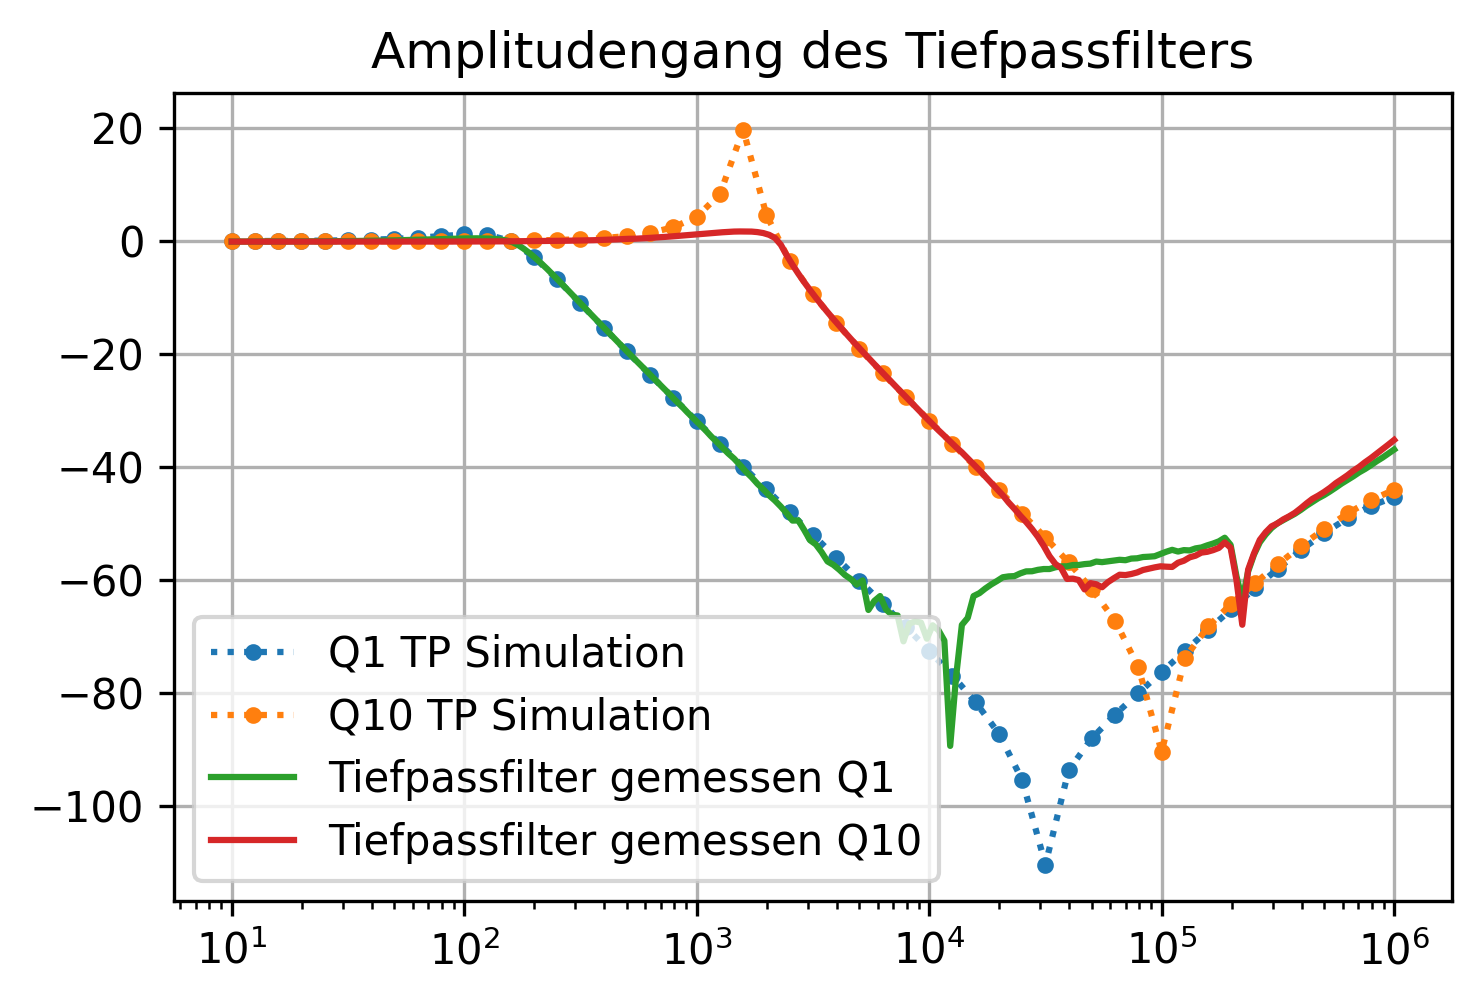
\includegraphics[keepaspectratio]{index_files/figure-pdf/cell-5-output-1.png}}

\subsection{Vergleich der Messwerte mit den
Simulationswerten}\label{vergleich-der-messwerte-mit-den-simulationswerten}

Vergleicht man die in Abbildung 2 abgebildeten Amplitudengände des
Tiefpassfilters, erkennt man ab ca. 10kHz bei Güte 1, bzw. 50kHz bei
Güte 10, Abweichungen der gemessenen zu der theoretischen Simulation aus
KiCad. Bei höheren Frequenzen kommen mehrerere Faktoren zusammen, die
das ideale Verhalten beeinträchtigen: - Parasitäre Effekte: Bei den
theoretischen Modellen werden die Streukapazitäten und -induktivitäten,
die in den realen Bauelementen vorhanden sind, nicht berücksichtigt.
Diese parasiäten Effekten werden aber bei hohen Frequenzen zunehmend
relevant und könnten einer der Faktoren der Abweichungen sein. -
Frequenzabhängiges Bauteilverhalten: Mit steigender Frequenz sinkt der
Widerstand vom Kondensator. Bei steigender Frequenz ändert sich damit
das Spannungsverhältnis, was zu Abweichungen führt. - Nicht-idealen
Eigenschaften eines OpAmps: Zum Beispiel die endliche Verstärkung,
Offsetspannungen und Eingangs-Bias-Ströme, haben potenziell die größten
Auswirkungen auf die Leistung eines Biquad-Filters. Diese Fehlerquellen
können zu Verzerrungen, Verlust der Genauigkeit und Fehlern in der
Frequenzgangkurve führen. Besonders bei präzisen Filtern und
Anwendungen, die eine exakte Frequenzantwort erfordern (z.\,B. Audio-
oder Kommunikationssysteme), müssen diese nicht-idealen Effekte
berücksichtigt und in der Schaltungs- oder Filtergestaltung ausgeglichen
werden.Um diese Probleme zu minimieren, wird in der Praxis häufig
Präzisions-OpAmps verwendet, die geringe Fehlerquellen aufweise

\subsection{Dokumentierte
Abweichungen}\label{dokumentierte-abweichungen}

In den Versuchsergebnissen wurden bereits erhebliche Abweichungen
zwischen berechneten und gemessenen Werten dokumentiert: - Die
Abweichungen der Grenzfrequenz beträgt 1,57kHz bzw. 15,8\% - Die
absolute Abweichung zwischen ReÜberschwingen im Übergangsbereich: Im
Bereich um 1000 Hz zeigt insbesondere die Q10-Simulation (orange) ein
deutliches Überschwingen, das beim Q10-Wert mit seiner steileren
Flankensteilheit zu erwarten ist

\subsection{Spezielle Effekte bei hohen
Frequenzen}\label{spezielle-effekte-bei-hohen-frequenzen}

Bei Frequenzen deutlich über der Grenzfrequenz kommen zusätzliche
Effekte zum Tragen: - Die Filtersteilheit realer Filter kann von den
theoretischen abweichen. - Belastungseffekte durch nachfolgeden Stufen
verändern die Filtercharakteristik. Wenn beispielsweise ein Hochpass an
einen Tiefpass angeschlossen wird, verändert sich das
Übertragungsverhalten durch die Parallelschaltung. Diese Beobachtungen
decken sich mit der Grafik, die deutliche Unterschiede zwischen
Suimulation und Messung im Breich ab 10kHz zeigt, insbesondere bei der
Tiefe der Dämpfungskurve und dem erneuten Anstieg bei sehr hohen
Frequenzen.

\begin{Shaded}
\begin{Highlighting}[]
\NormalTok{plt.figure(}\StringTok{"Phasengang des Tiefpass filters"}\NormalTok{)}
\NormalTok{plt.title(}\StringTok{"Phasengang des Tiefpass filters"}\NormalTok{)}
\NormalTok{plt.plot(f1,np.degrees(np.angle(Vlpf1)),}\StringTok{".:"}\NormalTok{,label}\OperatorTok{=}\StringTok{"Q1 TP Simulation"}\NormalTok{)}
\NormalTok{plt.plot(f2,np.degrees(np.angle(Vlpf10)),}\StringTok{".:"}\NormalTok{,label}\OperatorTok{=}\StringTok{"Q10 TP Simulation"}\NormalTok{)}
\NormalTok{plt.plot(fTPQ1,phaseTPQ1,}\StringTok{".:"}\NormalTok{,label}\OperatorTok{=}\StringTok{\textquotesingle{}Tiefpassfilter gemessen Q1\textquotesingle{}}\NormalTok{)}
\NormalTok{plt.plot(fTPQ10,phaseTPQ10,}\StringTok{".:"}\NormalTok{,label}\OperatorTok{=}\StringTok{\textquotesingle{}Tiefpassfilter gemessen Q10\textquotesingle{}}\NormalTok{)}
\NormalTok{plt.xscale(}\StringTok{\textquotesingle{}log\textquotesingle{}}\NormalTok{)}
\NormalTok{plt.grid()}
\NormalTok{plt.legend()}
\NormalTok{plt.show()}
\end{Highlighting}
\end{Shaded}

\pandocbounded{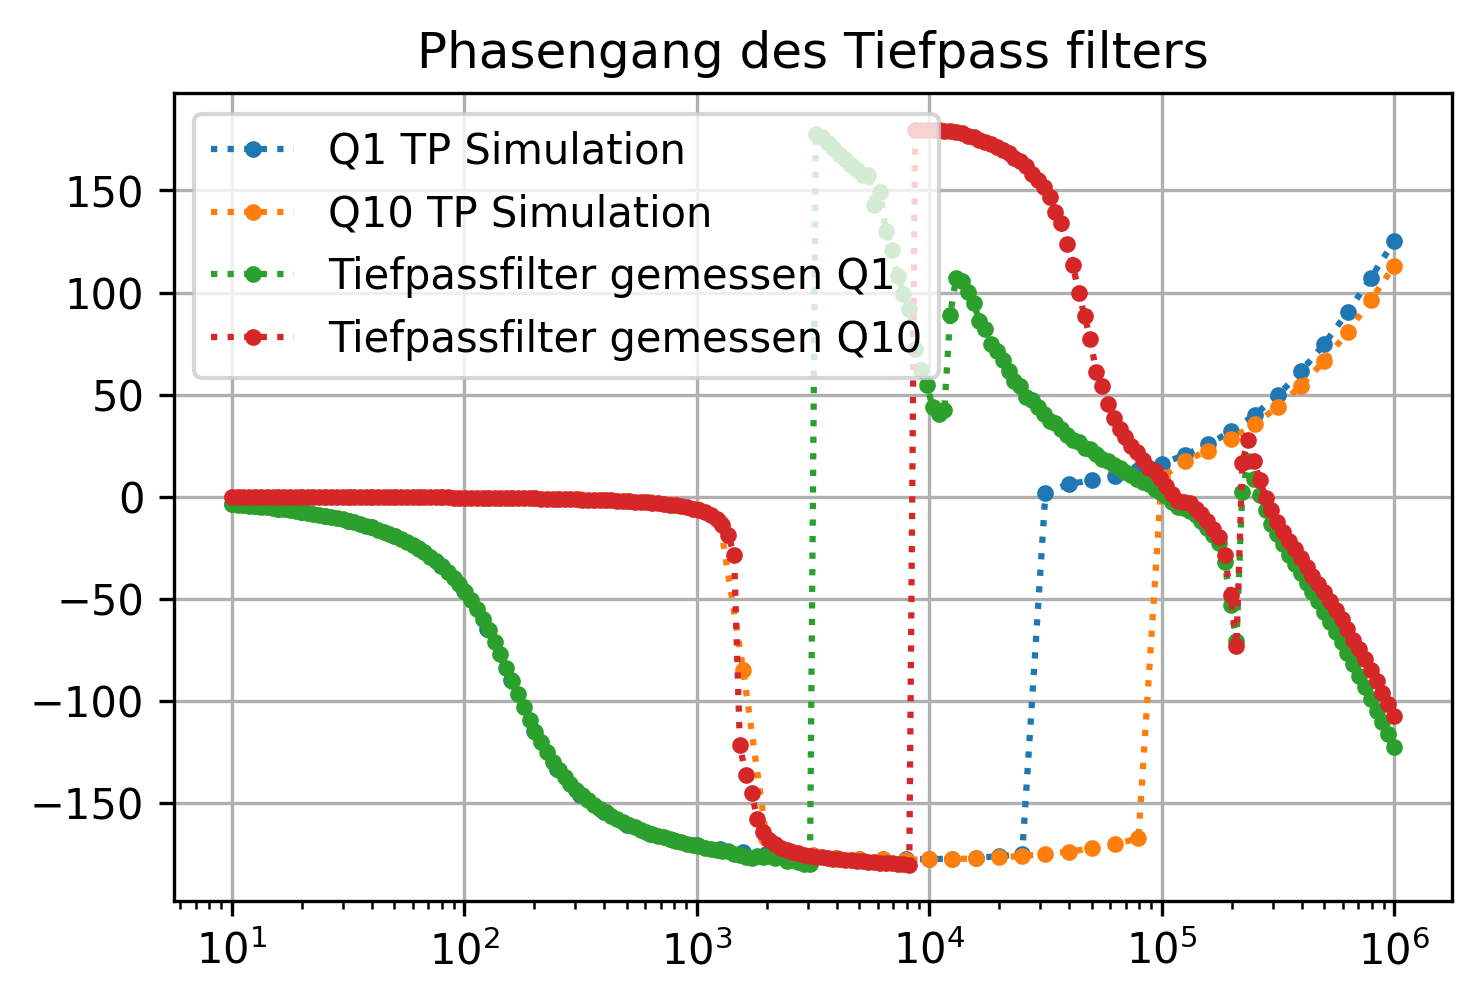
\includegraphics[keepaspectratio]{index_files/figure-pdf/cell-6-output-1.png}}

\section{Hochpassfilter}\label{hochpassfilter}

\begin{Shaded}
\begin{Highlighting}[]
\NormalTok{plt.figure(}\StringTok{"Amplitudengang des Hochpassfilters"}\NormalTok{)}
\NormalTok{plt.title(}\StringTok{"Amplitudengang des Hochpassfilters"}\NormalTok{)}
\NormalTok{plt.plot(f1,}\DecValTok{20}\OperatorTok{*}\NormalTok{np.log10(}\BuiltInTok{abs}\NormalTok{(Vhpf1)),}\StringTok{".:"}\NormalTok{,label}\OperatorTok{=}\StringTok{"Q1 HP Simulation"}\NormalTok{)}
\NormalTok{plt.plot(f2,}\DecValTok{20}\OperatorTok{*}\NormalTok{np.log10(}\BuiltInTok{abs}\NormalTok{(Vhpf10)),}\StringTok{".:"}\NormalTok{,label}\OperatorTok{=}\StringTok{"Q10 HP Simulation"}\NormalTok{)}
\NormalTok{plt.plot(fHPFQ1,gainHPFQ1,label}\OperatorTok{=}\StringTok{\textquotesingle{}Hochpassfilter gemessen Q1\textquotesingle{}}\NormalTok{)}
\NormalTok{plt.plot(fHPFQ10,gainHPFQ10,label}\OperatorTok{=}\StringTok{\textquotesingle{}Hochpassfilter gemessen Q10\textquotesingle{}}\NormalTok{)}
\NormalTok{plt.xscale(}\StringTok{\textquotesingle{}log\textquotesingle{}}\NormalTok{)}
\NormalTok{plt.grid()}
\NormalTok{plt.legend()}
\NormalTok{plt.show()}
\end{Highlighting}
\end{Shaded}

\pandocbounded{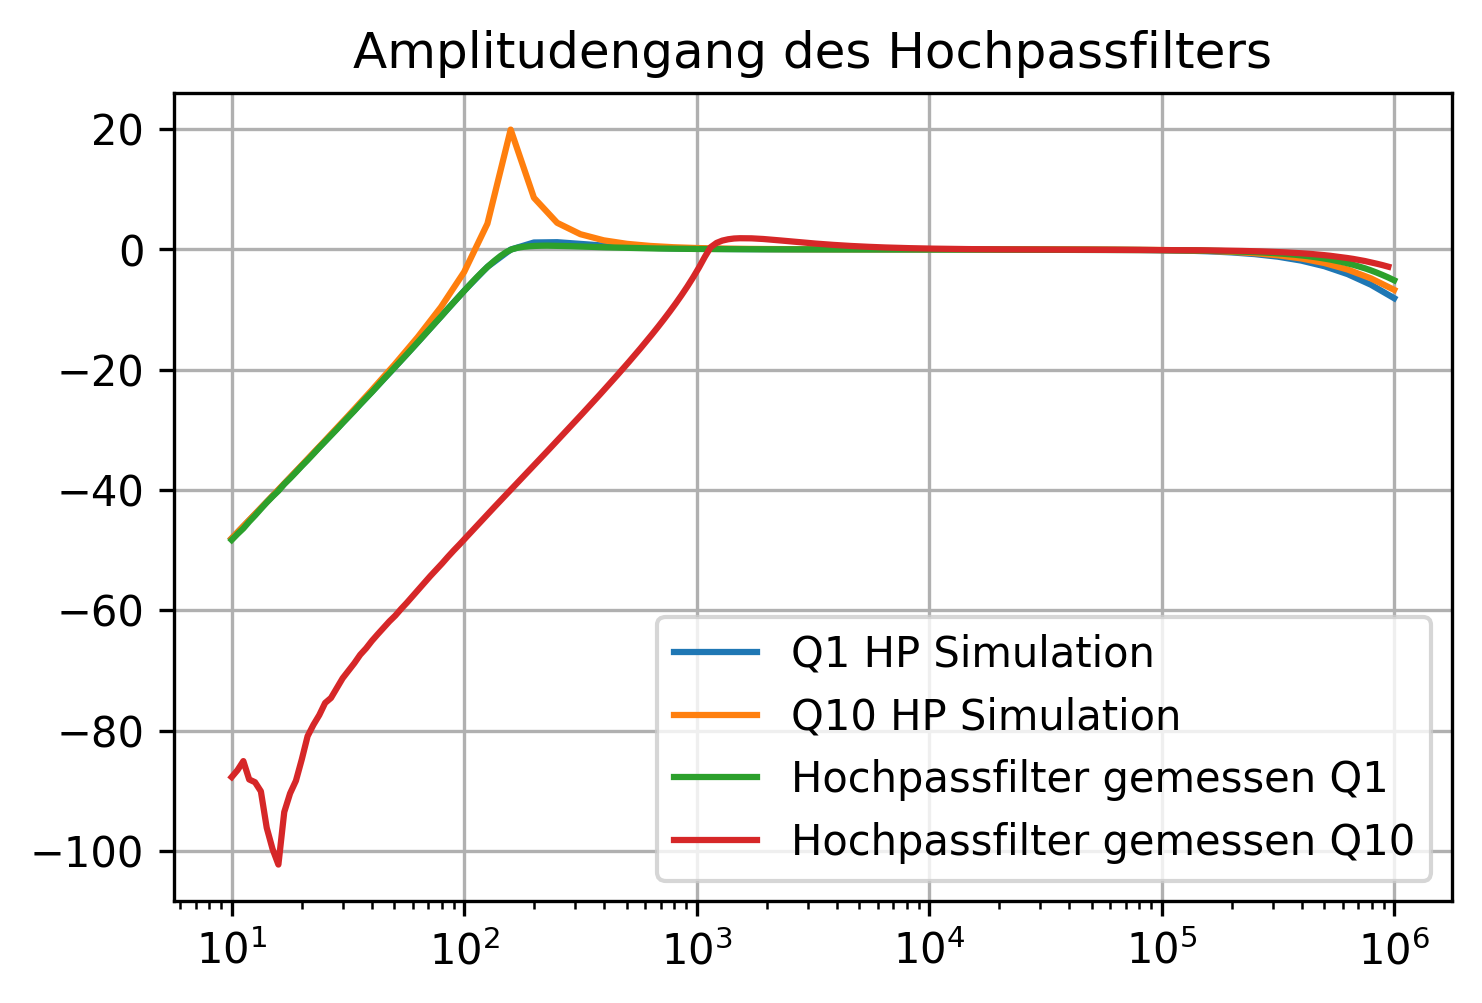
\includegraphics[keepaspectratio]{index_files/figure-pdf/cell-7-output-1.png}}

\subsection{Vergleich der Messwerte mit den
Simulationswerten}\label{vergleich-der-messwerte-mit-den-simulationswerten-1}

Bei den Amplitudengänge des Hochpassfilters aus Abbildung 4 gibt es
ähnliche Gründe für die Abweichungen wie beim Tiefpassfilter, aber mit
dem Unterschied, dass sie hier bei sehr niedrigen Frequenzen und
ebenfalls sehr niedrigen dB-Werten auftreten. Dabei gibt es mehrere
Faktoren, die diese Abweichungen erklären: - Reales Verhalten der
Bauelemente: Bei extrem niedrigen Frequenzen verhalten sich
Kondensatoren nicht mehr ideal. Während ein idealer Kondensator bei sehr
niedrigen Frequenzen wie eine vollständige Sperre wirken sollte, haben
reale Kondensatoren Leckströme, die einen gewissen Signaldurchlass
ermöglichen - Parasitäre Effekte: Reale Bauteile besitzen
Parallelwiderstände, die besonders bei niedrigen Frequenzen zum Tragen
kommen. Bei Kondensatoren führt dies dazu, dass sie nicht mehr als
perfekte Isolatoren wirken - Rauscheffekte und Messgenauigkeit: Bei sehr
niedirgen dB-Werten (unter -80dB) stoßen Messgeräte an ihre Grenzen, was
zu unregelmäßigen Messergebnissen führen kann.

\subsection{Dokumentierte
Abweichungen}\label{dokumentierte-abweichungen-1}

Im angezeigten Amplitudengang des Hochpassfilters sind mehrere
charakteristische Abweichungen erkennbar: - Starker Einbruch bei
Q1-Messung: Die rote Linie (gemessener Q1-Hochpass) zeigt bei etwa 20-30
Hz einen markanten Einbruch auf fast -110 dB, der in der Simulation
nicht vorkommt. Dies deutet auf resonante Effekte zwischen den realen
Bauteilen hin - Flacherer Anstieg bei niedrigen Frequenzen: Der Anstieg
der gemessenen Kurven (rot und grün) ist bei sehr niedrigen Frequenzen
weniger steil als bei den simulierten Kurven, was auf die nicht-idealen
Eigenschaften der Bauelemente zurückzuführen ist - Überschwingen im
Übergangsbereich: Im Bereich um 1000 Hz zeigt insbesondere die
Q10-Simulation (orange) ein deutliches Überschwingen, das beim Q10-Wert
mit seiner steileren Flankensteilheit zu erwarten ist

\begin{Shaded}
\begin{Highlighting}[]
\NormalTok{plt.figure(}\StringTok{"Phasengang des Hochpassfilters"}\NormalTok{)}
\NormalTok{plt.title(}\StringTok{"Phasengang des Hochpassfilters"}\NormalTok{)}
\NormalTok{plt.plot(f1,np.degrees(np.angle(Vhpf1)),}\StringTok{".:"}\NormalTok{,label}\OperatorTok{=}\StringTok{"Q1 HP Simulation"}\NormalTok{)}
\NormalTok{plt.plot(f2,np.degrees(np.angle(Vhpf10)),}\StringTok{".:"}\NormalTok{,label}\OperatorTok{=}\StringTok{"Q10 HP Simulation"}\NormalTok{)}
\NormalTok{plt.plot(fHPFQ1,phaseHPFQ1,label}\OperatorTok{=}\StringTok{\textquotesingle{}Hochpassfilter gemessen Q1\textquotesingle{}}\NormalTok{)}
\NormalTok{plt.plot(fHPFQ10,phaseHPFQ10,label}\OperatorTok{=}\StringTok{\textquotesingle{}Hochpassfilter gemessen Q10\textquotesingle{}}\NormalTok{)}
\NormalTok{plt.xscale(}\StringTok{\textquotesingle{}log\textquotesingle{}}\NormalTok{)}
\NormalTok{plt.grid()}
\NormalTok{plt.legend()}
\NormalTok{plt.show()}
\end{Highlighting}
\end{Shaded}

\pandocbounded{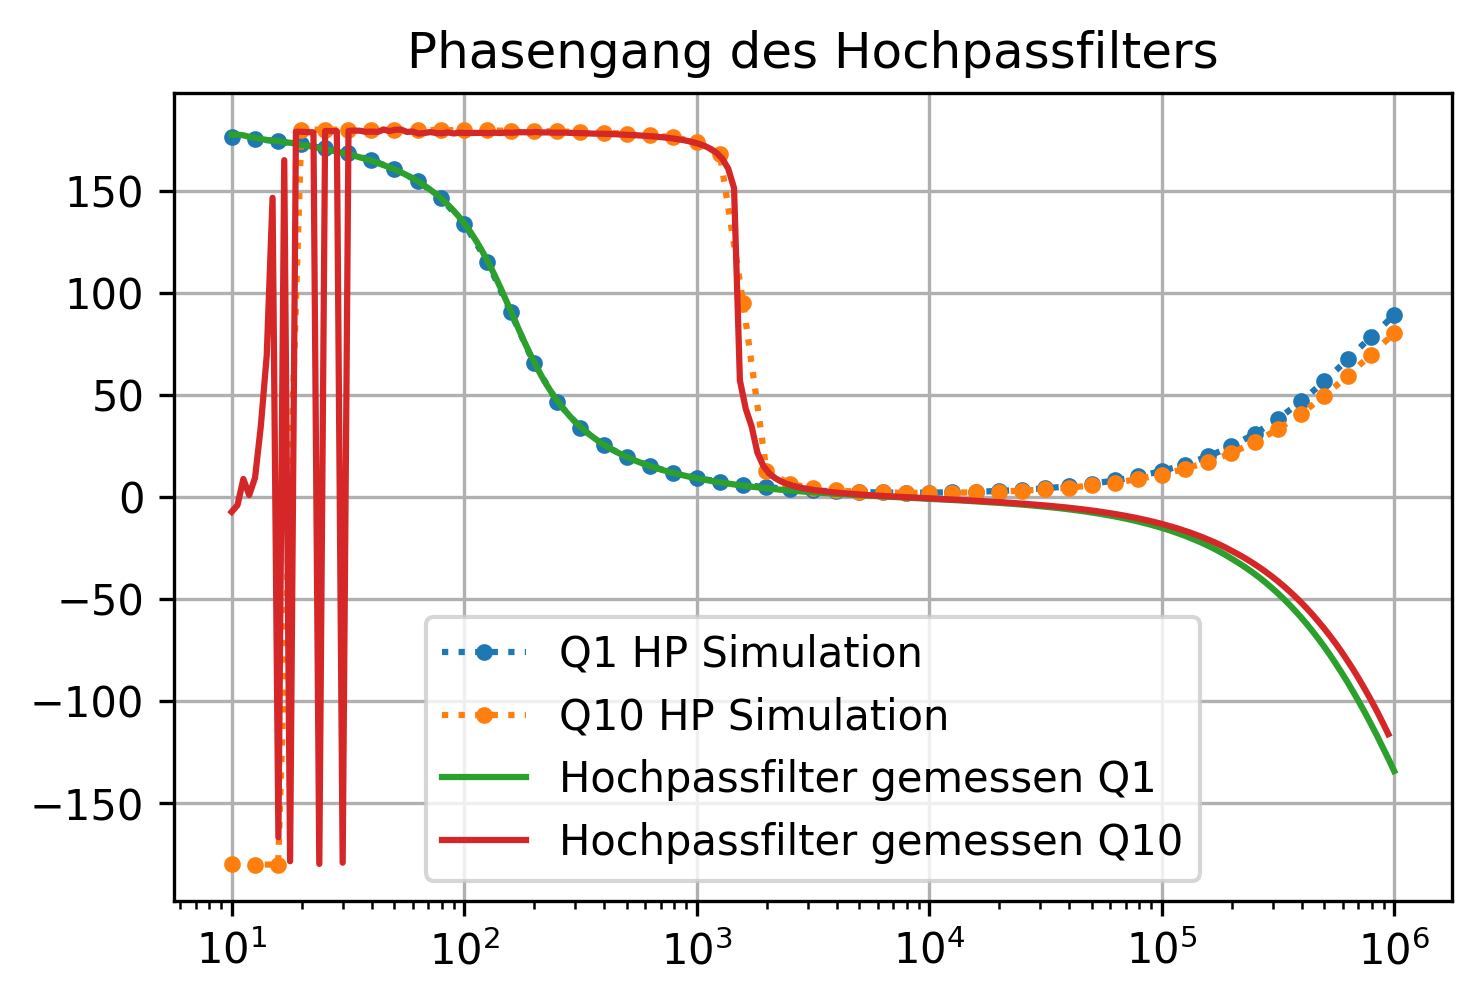
\includegraphics[keepaspectratio]{index_files/figure-pdf/cell-8-output-1.png}}

\section{Bandpassfilter}\label{bandpassfilter}

\begin{Shaded}
\begin{Highlighting}[]
\NormalTok{plt.figure(}\StringTok{"Amplitudengang des Bandpassfilters"}\NormalTok{)}
\NormalTok{plt.title(}\StringTok{"Amplitudengang des Bandpassfilters"}\NormalTok{)}
\NormalTok{plt.plot(f1,}\DecValTok{20}\OperatorTok{*}\NormalTok{np.log10(}\BuiltInTok{abs}\NormalTok{(Vbpf1)),}\StringTok{".:"}\NormalTok{,label}\OperatorTok{=}\StringTok{"https://www.ti.com/lit/ds/symlink/tl082{-}n.pdfQ1 BPF Simulation"}\NormalTok{)}
\NormalTok{plt.plot(f2,}\DecValTok{20}\OperatorTok{*}\NormalTok{np.log10(}\BuiltInTok{abs}\NormalTok{(Vbpf10)),}\StringTok{".:"}\NormalTok{,label}\OperatorTok{=}\StringTok{"Q10 BPF Simulation"}\NormalTok{)}
\NormalTok{plt.plot(fBPFQ1,gainBPFQ1,label}\OperatorTok{=}\StringTok{\textquotesingle{}Bandpassfilter gemessen Q1\textquotesingle{}}\NormalTok{)}
\NormalTok{plt.plot(fBPFQ10,gainBPFQ10,label}\OperatorTok{=}\StringTok{\textquotesingle{}Bandpassfilter gemessen Q10\textquotesingle{}}\NormalTok{)}
\NormalTok{plt.xscale(}\StringTok{\textquotesingle{}log\textquotesingle{}}\NormalTok{)}
\NormalTok{plt.grid()}
\NormalTok{plt.legend()}
\NormalTok{plt.show()}
\end{Highlighting}
\end{Shaded}

\pandocbounded{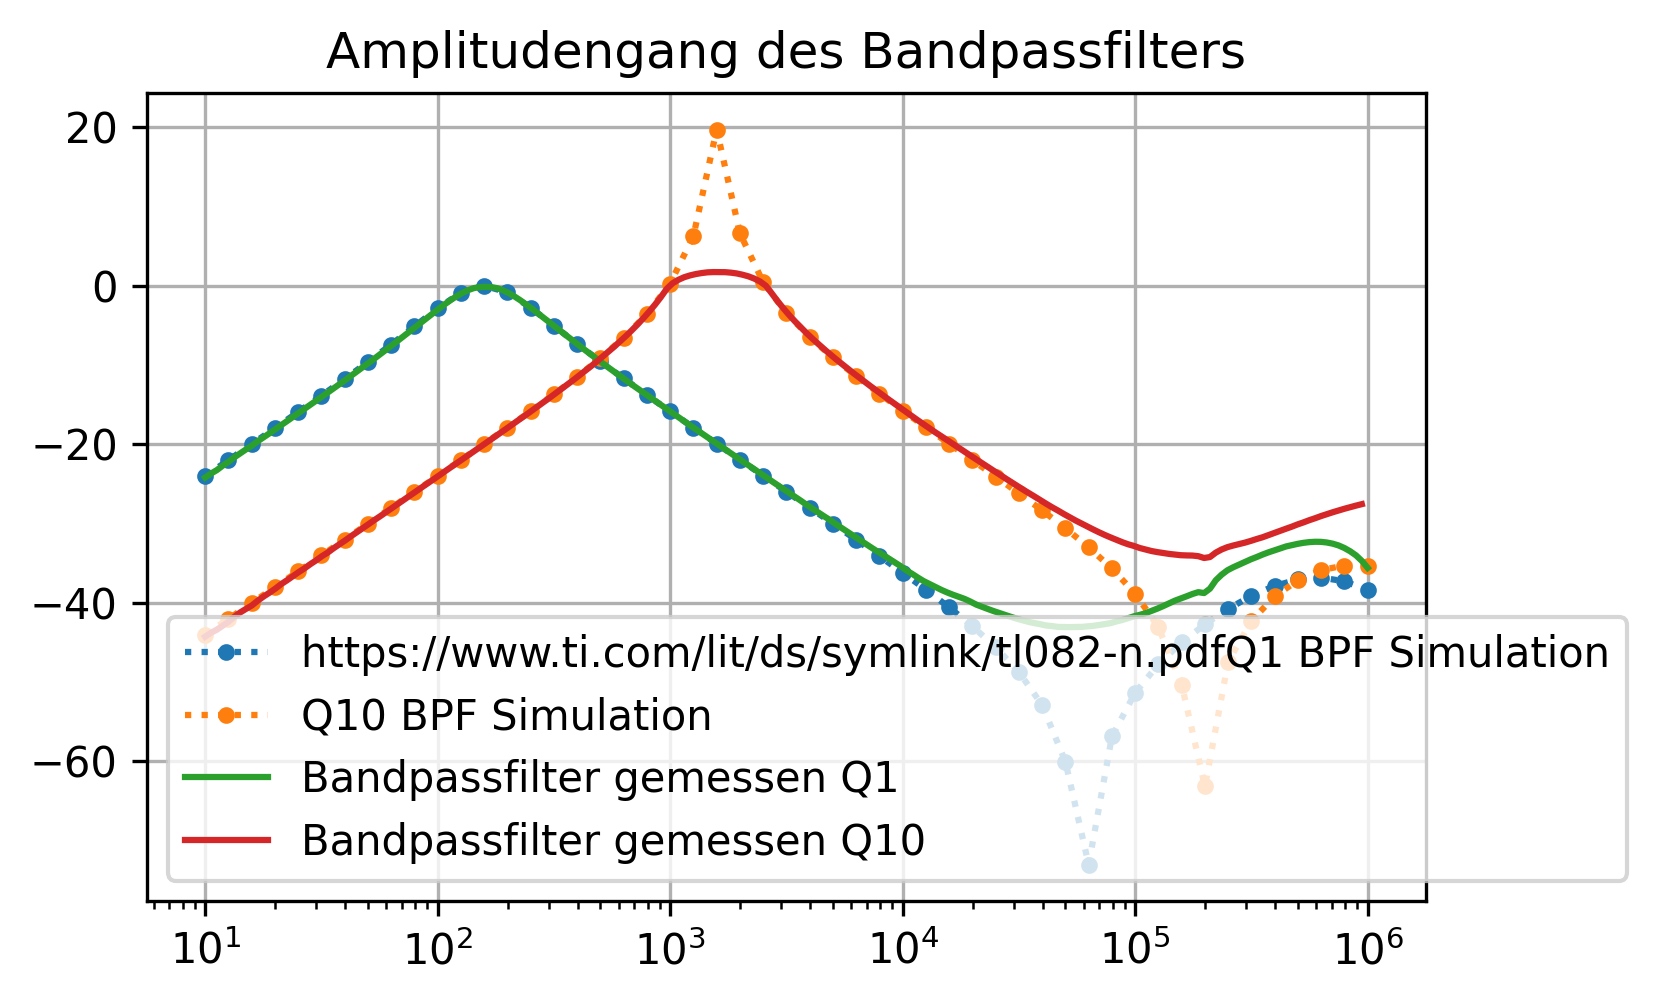
\includegraphics[keepaspectratio]{index_files/figure-pdf/cell-9-output-1.png}}

\begin{Shaded}
\begin{Highlighting}[]
\NormalTok{plt.figure(}\StringTok{"Phasengang des Bandpassfilters"}\NormalTok{)}
\NormalTok{plt.title(}\StringTok{"Phasengang des Bandpassfilters"}\NormalTok{)}
\NormalTok{plt.plot(f1,np.degrees(np.angle(Vbpf1)),}\StringTok{".:"}\NormalTok{,label}\OperatorTok{=}\StringTok{"Q1 BPF Simulation"}\NormalTok{)}
\NormalTok{plt.plot(f2,np.degrees(np.angle(Vbpf10)),}\StringTok{".:"}\NormalTok{,label}\OperatorTok{=}\StringTok{"Q10 BPF Simulation"}\NormalTok{)}
\NormalTok{plt.plot(fBPFQ1,phaseBPFQ1,label}\OperatorTok{=}\StringTok{\textquotesingle{}Bandpassfilter gemessen Q1\textquotesingle{}}\NormalTok{)}
\NormalTok{plt.plot(fBPFQ10,phaseBPFQ10,label}\OperatorTok{=}\StringTok{\textquotesingle{}Bandpassfilter gemessen Q10\textquotesingle{}}\NormalTok{)}
\NormalTok{plt.xscale(}\StringTok{\textquotesingle{}log\textquotesingle{}}\NormalTok{)}
\NormalTok{plt.grid()}
\NormalTok{plt.legend()}
\NormalTok{plt.show()}
\end{Highlighting}
\end{Shaded}

\pandocbounded{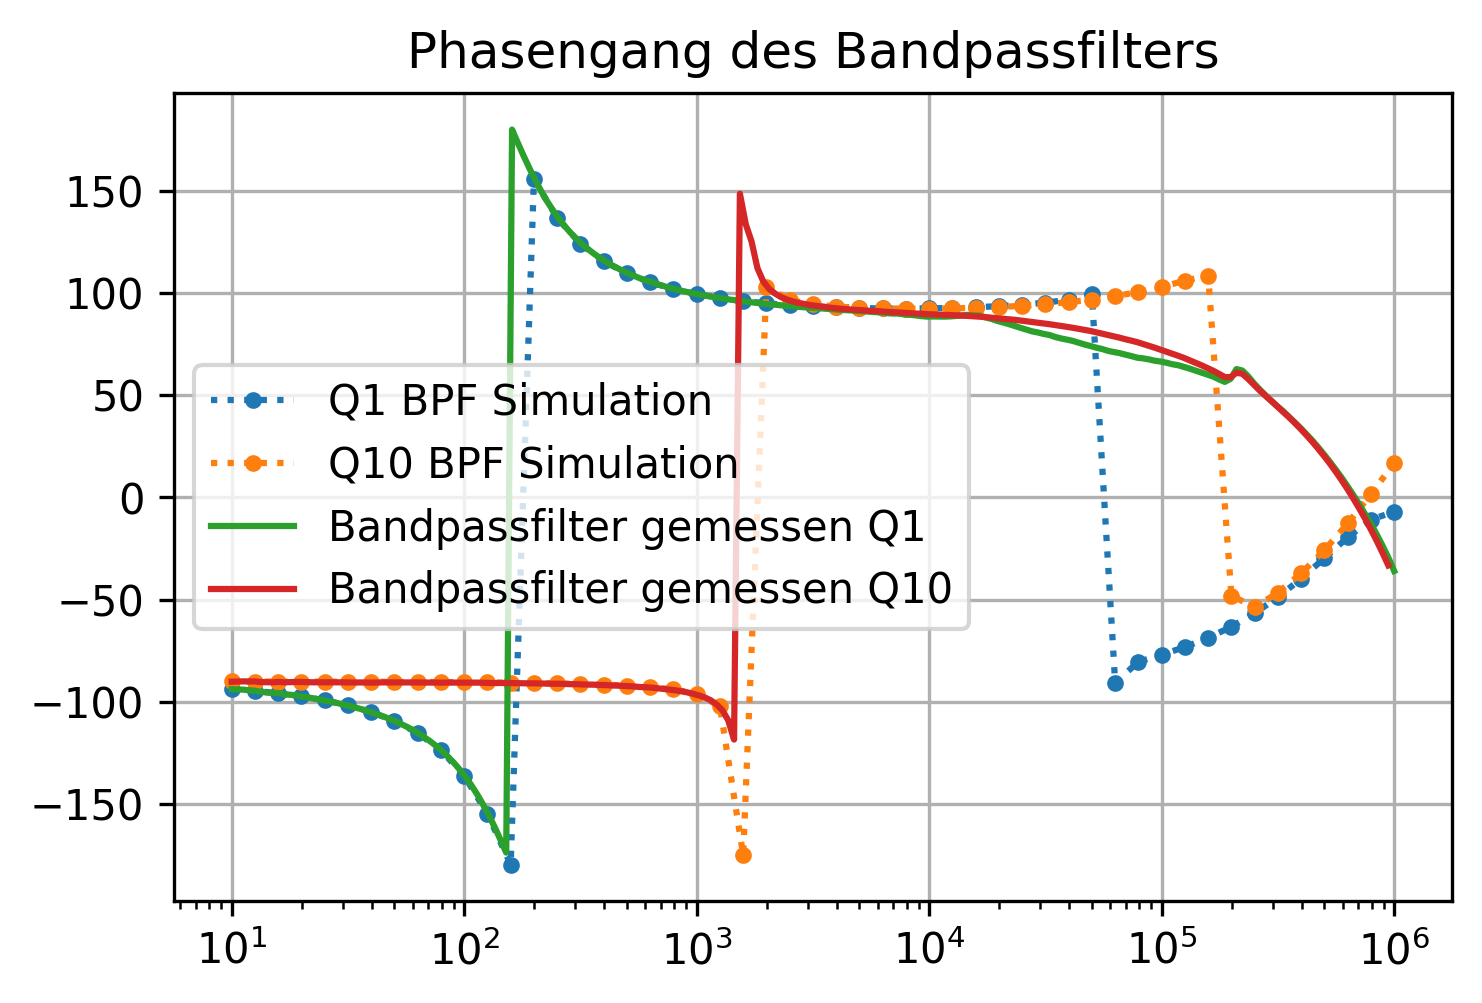
\includegraphics[keepaspectratio]{index_files/figure-pdf/cell-10-output-1.png}}

\section{Bandstopfilter}\label{bandstopfilter}

\begin{Shaded}
\begin{Highlighting}[]
\NormalTok{plt.figure(}\StringTok{"Amplitudengang des Bandstopfilters"}\NormalTok{)}
\NormalTok{plt.title(}\StringTok{"Amplitudengang des Bandstopfilters"}\NormalTok{)}
\NormalTok{plt.plot(f1,}\DecValTok{20}\OperatorTok{*}\NormalTok{np.log10(}\BuiltInTok{abs}\NormalTok{(Vbsf1)),}\StringTok{".:"}\NormalTok{,label}\OperatorTok{=}\StringTok{"Q1 BSF Simulation"}\NormalTok{)}
\NormalTok{plt.plot(f2,}\DecValTok{20}\OperatorTok{*}\NormalTok{np.log10(}\BuiltInTok{abs}\NormalTok{(Vbsf10)),}\StringTok{".:"}\NormalTok{,label}\OperatorTok{=}\StringTok{"Q10 BSF Simulation"}\NormalTok{)}
\NormalTok{plt.plot(fBSFQ1,gainBSFQ1,label}\OperatorTok{=}\StringTok{\textquotesingle{}Bandstopfilter gemessen Q1\textquotesingle{}}\NormalTok{)}
\NormalTok{plt.plot(fBSFQ10,gainBSFQ10,label}\OperatorTok{=}\StringTok{\textquotesingle{}Bandstopfilter gemessen Q10\textquotesingle{}}\NormalTok{)}
\NormalTok{plt.xscale(}\StringTok{\textquotesingle{}log\textquotesingle{}}\NormalTok{)}
\NormalTok{plt.grid()}
\NormalTok{plt.legend()}
\NormalTok{plt.show()}
\end{Highlighting}
\end{Shaded}

\pandocbounded{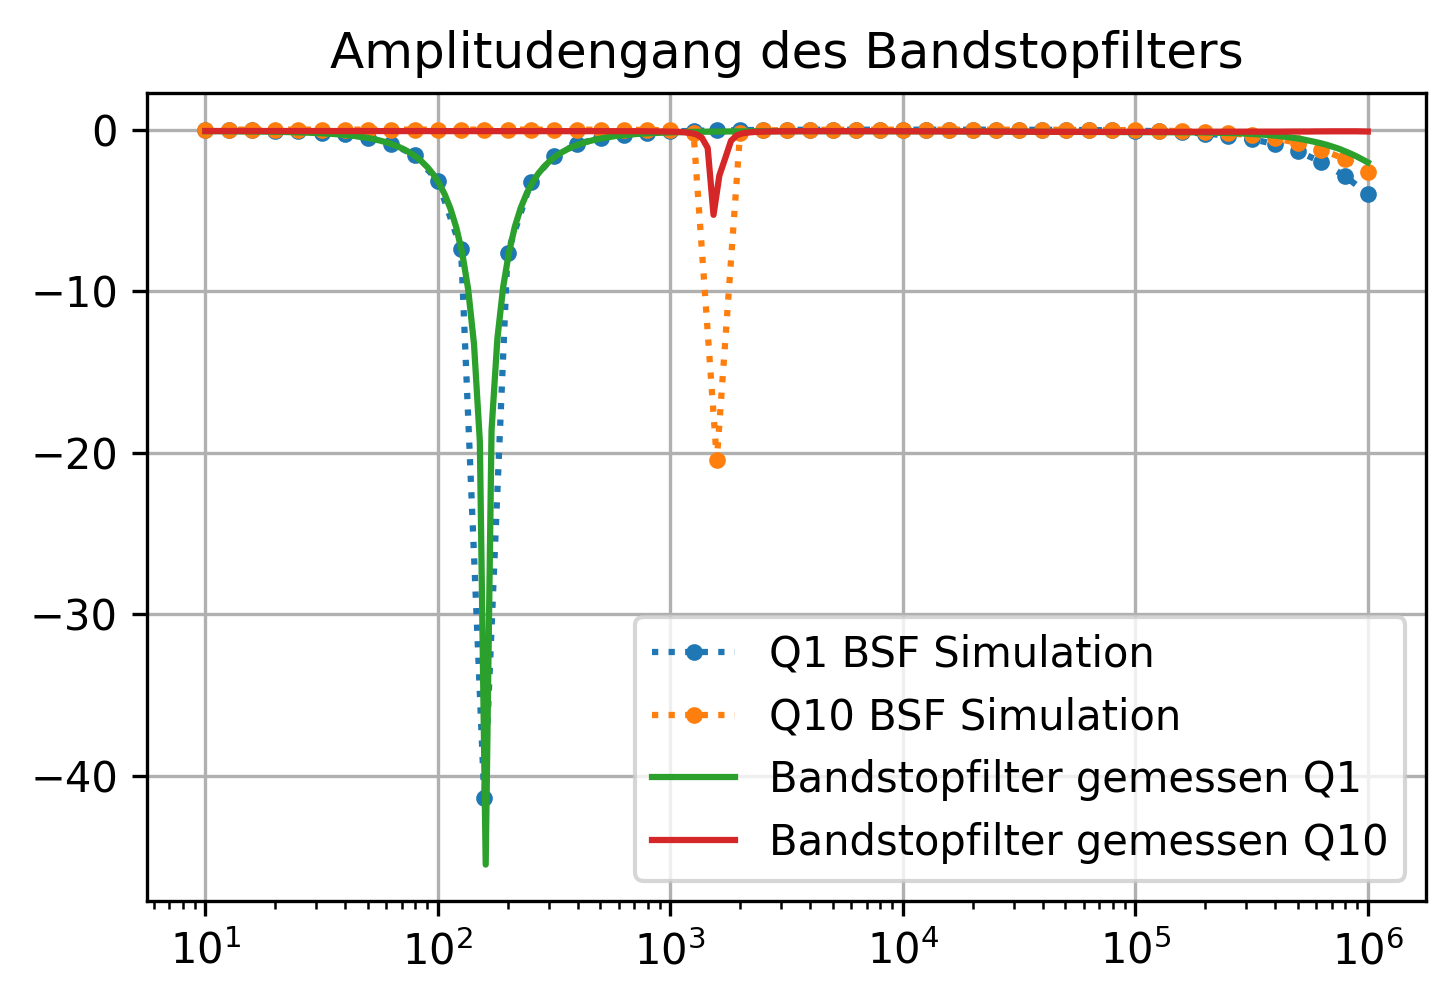
\includegraphics[keepaspectratio]{index_files/figure-pdf/cell-11-output-1.png}}

\begin{Shaded}
\begin{Highlighting}[]
\NormalTok{plt.figure(}\StringTok{"Phasengang des Bandstopfilters"}\NormalTok{)}
\NormalTok{plt.title(}\StringTok{"Phasengang des Bandstopfilters"}\NormalTok{)}
\NormalTok{plt.plot(f1,np.degrees(np.angle(Vbsf1)),}\StringTok{".:"}\NormalTok{,label}\OperatorTok{=}\StringTok{"Q1 BSF Simulation"}\NormalTok{)}
\NormalTok{plt.plot(f2,np.degrees(np.angle(Vbsf10)),}\StringTok{".:"}\NormalTok{,label}\OperatorTok{=}\StringTok{"Q10 BSF Simulation"}\NormalTok{)}
\NormalTok{plt.plot(fBSFQ1,phaseBSFQ1,label}\OperatorTok{=}\StringTok{\textquotesingle{}Bandstopfilter gemessen Q1\textquotesingle{}}\NormalTok{)}
\NormalTok{plt.plot(fBSFQ10,phaseBSFQ10,label}\OperatorTok{=}\StringTok{\textquotesingle{}Bandstopfilter gemessen Q10\textquotesingle{}}\NormalTok{)}
\NormalTok{plt.xscale(}\StringTok{\textquotesingle{}log\textquotesingle{}}\NormalTok{)}
\NormalTok{plt.grid()}
\NormalTok{plt.legend()}
\NormalTok{plt.show()}
\end{Highlighting}
\end{Shaded}

\pandocbounded{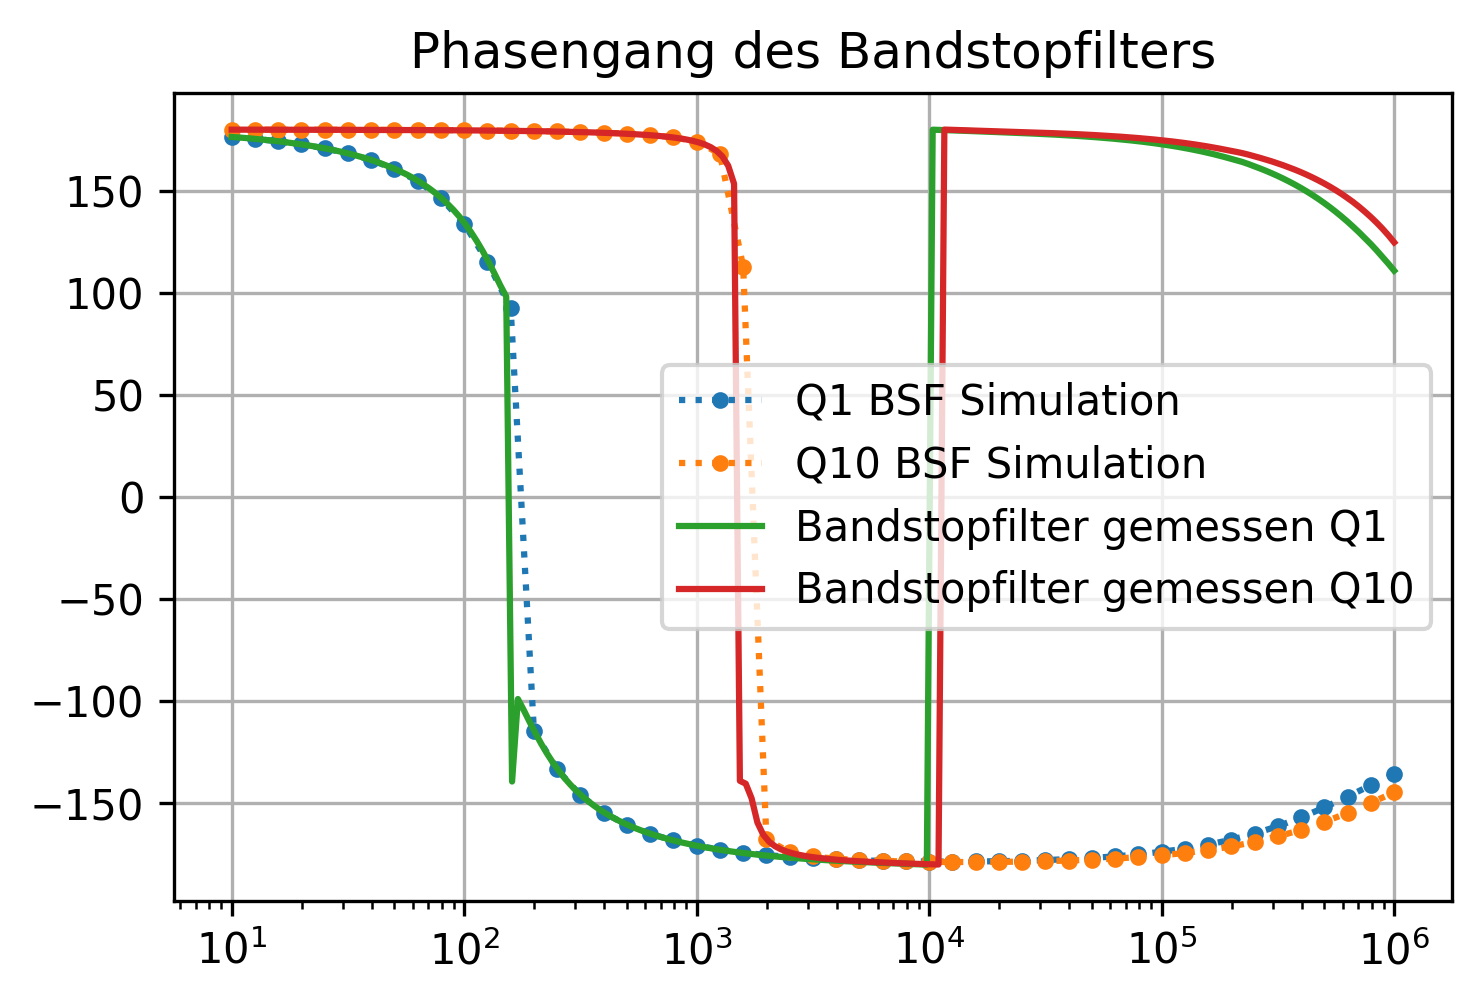
\includegraphics[keepaspectratio]{index_files/figure-pdf/cell-12-output-1.png}}

Die Güte hat ein Problem in der Rellen Schaltung

\chapter{Butterworthfilter}\label{butterworthfilter}

\begin{Shaded}
\begin{Highlighting}[]
\CommentTok{\# Einladen der Messwerte}
\CommentTok{\# {-}{-}{-}{-}{-} Butter1uF {-}{-}{-}{-}{-}{-}{-}{-}{-}{-}{-}{-}{-} }
\NormalTok{Butter1uF }\OperatorTok{=}\NormalTok{ pd.read\_csv(}\StringTok{"./Data/4.5\_1uF\_Data.csv"}\NormalTok{,sep}\OperatorTok{=}\StringTok{\textquotesingle{},\textquotesingle{}}\NormalTok{)}
\NormalTok{fButter1uf }\OperatorTok{=}\NormalTok{ np.array(Butter1uF[}\StringTok{\textquotesingle{}Frequency [Hz]\textquotesingle{}}\NormalTok{])}
\NormalTok{gain1uf}\OperatorTok{=}\NormalTok{np.array(Butter1uF[}\StringTok{\textquotesingle{} Amplitude [dB]\textquotesingle{}}\NormalTok{])}
\NormalTok{phase1uf }\OperatorTok{=}\NormalTok{ np.array(Butter1uF[}\StringTok{\textquotesingle{} Phase [deg]\textquotesingle{}}\NormalTok{])}

\CommentTok{\# {-}{-}{-}{-}{-}{-}Butter 0.1 uF {-}{-}{-}{-}{-}{-}{-}{-}{-}{-} }
\NormalTok{Butter01uF }\OperatorTok{=}\NormalTok{ pd.read\_csv(}\StringTok{"./Data/4.5\_0.1uF\_Data.csv"}\NormalTok{,sep}\OperatorTok{=}\StringTok{\textquotesingle{},\textquotesingle{}}\NormalTok{)}
\NormalTok{fButter01uf }\OperatorTok{=}\NormalTok{ np.array(Butter01uF[}\StringTok{\textquotesingle{}Frequency [Hz]\textquotesingle{}}\NormalTok{])}
\NormalTok{gain01uf}\OperatorTok{=}\NormalTok{np.array(Butter01uF[}\StringTok{\textquotesingle{} Amplitude [dB]\textquotesingle{}}\NormalTok{])}
\NormalTok{phase01uf }\OperatorTok{=}\NormalTok{ np.array(Butter01uF[}\StringTok{\textquotesingle{} Phase [deg]\textquotesingle{}}\NormalTok{])}

\CommentTok{\# {-}{-}{-}{-}{-}{-}Butter 0.01uF {-}{-}{-}{-}{-}{-}{-}{-} f0 = }
\NormalTok{Butter001uF }\OperatorTok{=}\NormalTok{ pd.read\_csv(}\StringTok{"./Data/4.5\_0.01uf\_Data.csv"}\NormalTok{,sep}\OperatorTok{=}\StringTok{\textquotesingle{},\textquotesingle{}}\NormalTok{)}
\NormalTok{fButter001uf }\OperatorTok{=}\NormalTok{ np.array(Butter001uF[}\StringTok{\textquotesingle{}Frequency [Hz]\textquotesingle{}}\NormalTok{])}
\NormalTok{gain001uf}\OperatorTok{=}\NormalTok{np.array(Butter001uF[}\StringTok{\textquotesingle{} Amplitude [dB]\textquotesingle{}}\NormalTok{])}
\NormalTok{phase001uf }\OperatorTok{=}\NormalTok{ np.array(Butter001uF[}\StringTok{\textquotesingle{} Phase [deg]\textquotesingle{}}\NormalTok{])}
\end{Highlighting}
\end{Shaded}

\begin{Shaded}
\begin{Highlighting}[]
\CommentTok{\# Einladen der Simuliertenwerte}

\CommentTok{\# Werte aus der Simulation mit 1 uF  }
\NormalTok{filepath3 }\OperatorTok{=} \StringTok{\textquotesingle{}./spice\_kicad/Butterworththirdorder1u.raw\textquotesingle{}}
\NormalTok{l3 }\OperatorTok{=}\NormalTok{ Ltspice(filepath3)}
\NormalTok{l3.parse() }\CommentTok{\# Data loading sequence. It may take few minutes for huge file.}

\NormalTok{f3 }\OperatorTok{=}\NormalTok{ l3.get\_frequency()}
\NormalTok{Vbpf3 }\OperatorTok{=}\NormalTok{ l3.get\_data(}\StringTok{\textquotesingle{}v(bpf)\textquotesingle{}}\NormalTok{)}
\NormalTok{Vbsf3 }\OperatorTok{=}\NormalTok{ l3.get\_data(}\StringTok{\textquotesingle{}v(bsf)\textquotesingle{}}\NormalTok{)}
\NormalTok{Vhpf3 }\OperatorTok{=}\NormalTok{ l3.get\_data(}\StringTok{\textquotesingle{}v(hpf)\textquotesingle{}}\NormalTok{)}
\NormalTok{Vlpf3 }\OperatorTok{=}\NormalTok{ l3.get\_data(}\StringTok{\textquotesingle{}v(lpf)\textquotesingle{}}\NormalTok{)}
\NormalTok{Vout1u  }\OperatorTok{=}\NormalTok{ l3.get\_data(}\StringTok{\textquotesingle{}v(Vout)\textquotesingle{}}\NormalTok{) }

\CommentTok{\# Werte aus der Simulation mit 0.1 uF}

\NormalTok{filepath4 }\OperatorTok{=} \StringTok{\textquotesingle{}./spice\_kicad/Butterworththirdorder0.1u.raw\textquotesingle{}}
\NormalTok{l4 }\OperatorTok{=}\NormalTok{ Ltspice(filepath4)}
\NormalTok{l4.parse() }\CommentTok{\# Data loading sequence. It may take few minutes for huge file.}

\NormalTok{f4 }\OperatorTok{=}\NormalTok{ l4.get\_frequency()}
\NormalTok{Vbpf4 }\OperatorTok{=}\NormalTok{ l4.get\_data(}\StringTok{\textquotesingle{}v(bpf)\textquotesingle{}}\NormalTok{)}
\NormalTok{Vbsf4 }\OperatorTok{=}\NormalTok{ l4.get\_data(}\StringTok{\textquotesingle{}v(bsf)\textquotesingle{}}\NormalTok{)}
\NormalTok{Vhpf4 }\OperatorTok{=}\NormalTok{ l4.get\_data(}\StringTok{\textquotesingle{}v(hpf)\textquotesingle{}}\NormalTok{)}
\NormalTok{Vlpf4 }\OperatorTok{=}\NormalTok{ l4.get\_data(}\StringTok{\textquotesingle{}v(lpf)\textquotesingle{}}\NormalTok{)}
\NormalTok{Vout01u  }\OperatorTok{=}\NormalTok{ l4.get\_data(}\StringTok{\textquotesingle{}v(Vout)\textquotesingle{}}\NormalTok{) }

\CommentTok{\# Werte aus der Simulation mit 0.01 uF}

\NormalTok{filepath5 }\OperatorTok{=} \StringTok{\textquotesingle{}./spice\_kicad/Butterworththirdorder0.01u.raw\textquotesingle{}}
\NormalTok{l5 }\OperatorTok{=}\NormalTok{ Ltspice(filepath5)}
\NormalTok{l5.parse() }\CommentTok{\# Data loading sequence. It may take few minutes for huge file.}

\NormalTok{f5 }\OperatorTok{=}\NormalTok{ l5.get\_frequency()}
\NormalTok{Vbpf5 }\OperatorTok{=}\NormalTok{ l5.get\_data(}\StringTok{\textquotesingle{}v(bpf)\textquotesingle{}}\NormalTok{)}
\NormalTok{Vbsf5 }\OperatorTok{=}\NormalTok{ l5.get\_data(}\StringTok{\textquotesingle{}v(bsf)\textquotesingle{}}\NormalTok{)}
\NormalTok{Vhpf5 }\OperatorTok{=}\NormalTok{ l5.get\_data(}\StringTok{\textquotesingle{}v(hpf)\textquotesingle{}}\NormalTok{)}
\NormalTok{Vlpf5 }\OperatorTok{=}\NormalTok{ l5.get\_data(}\StringTok{\textquotesingle{}v(lpf)\textquotesingle{}}\NormalTok{)}
\NormalTok{Vout001u  }\OperatorTok{=}\NormalTok{ l5.get\_data(}\StringTok{\textquotesingle{}v(Vout)\textquotesingle{}}\NormalTok{) }
\end{Highlighting}
\end{Shaded}

\section{Plot und Vergleich:}\label{plot-und-vergleich}

\subsection{Butterworth 1uF}\label{butterworth-1uf}

\begin{Shaded}
\begin{Highlighting}[]
\NormalTok{plt.figure(}\StringTok{"Amplitudengang Butterworth TP 1uF"}\NormalTok{)}
\NormalTok{plt.title(}\StringTok{"Amplitudengang Butterworth 1uF"}\NormalTok{)}
\NormalTok{plt.plot(f3,}\DecValTok{20}\OperatorTok{*}\NormalTok{np.log10(}\BuiltInTok{abs}\NormalTok{(Vout1u)),}\StringTok{".:"}\NormalTok{,label}\OperatorTok{=}\StringTok{"Simulation"}\NormalTok{)}
\NormalTok{plt.plot(fButter1uf,gain1uf,label}\OperatorTok{=}\StringTok{\textquotesingle{}Tiefpassfilter gemessen\textquotesingle{}}\NormalTok{)}
\NormalTok{plt.xscale(}\StringTok{\textquotesingle{}log\textquotesingle{}}\NormalTok{)}
\NormalTok{plt.grid()}
\NormalTok{plt.legend()}
\NormalTok{plt.show()}
\end{Highlighting}
\end{Shaded}

\pandocbounded{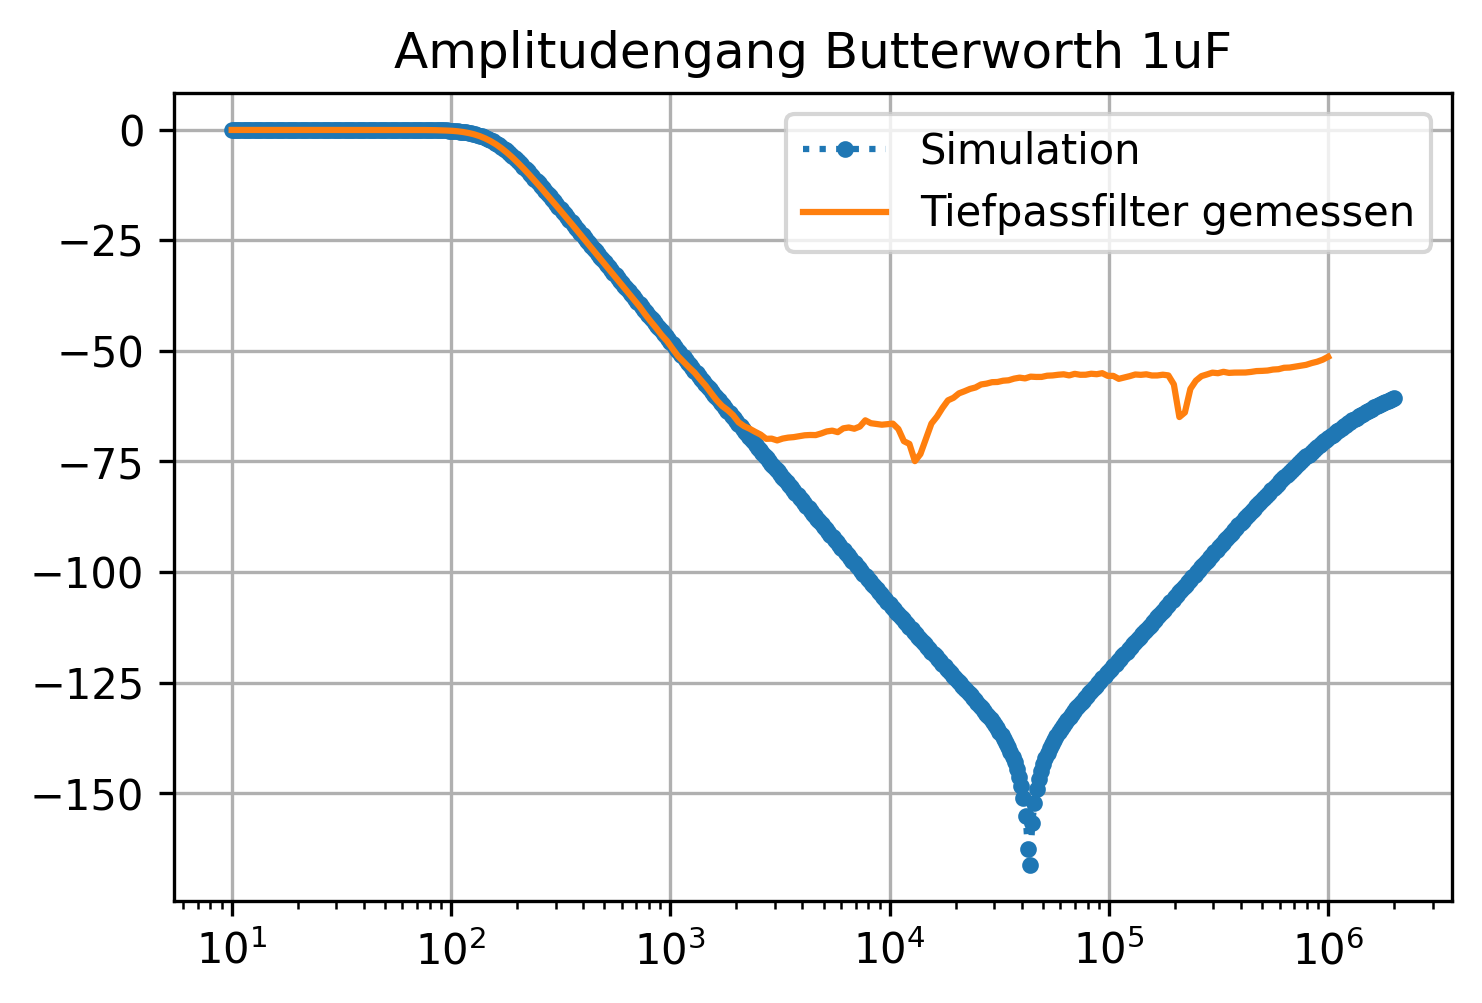
\includegraphics[keepaspectratio]{index_files/figure-pdf/cell-15-output-1.png}}

\begin{Shaded}
\begin{Highlighting}[]
\NormalTok{plt.figure(}\StringTok{"Phasengang Butterworth TP 1uF"}\NormalTok{)}
\NormalTok{plt.title(}\StringTok{"Phasengang Butterworth 1uF"}\NormalTok{)}
\NormalTok{plt.plot(f3,np.degrees(np.angle(Vout1u)),}\StringTok{".:"}\NormalTok{,label}\OperatorTok{=}\StringTok{"Simulation"}\NormalTok{)}
\NormalTok{plt.plot(fButter1uf,phase1uf,label}\OperatorTok{=}\StringTok{\textquotesingle{}Butterworth gemessen\textquotesingle{}}\NormalTok{)}
\NormalTok{plt.xscale(}\StringTok{\textquotesingle{}log\textquotesingle{}}\NormalTok{)}
\NormalTok{plt.grid()}
\NormalTok{plt.legend()}
\NormalTok{plt.show()}
\end{Highlighting}
\end{Shaded}

\pandocbounded{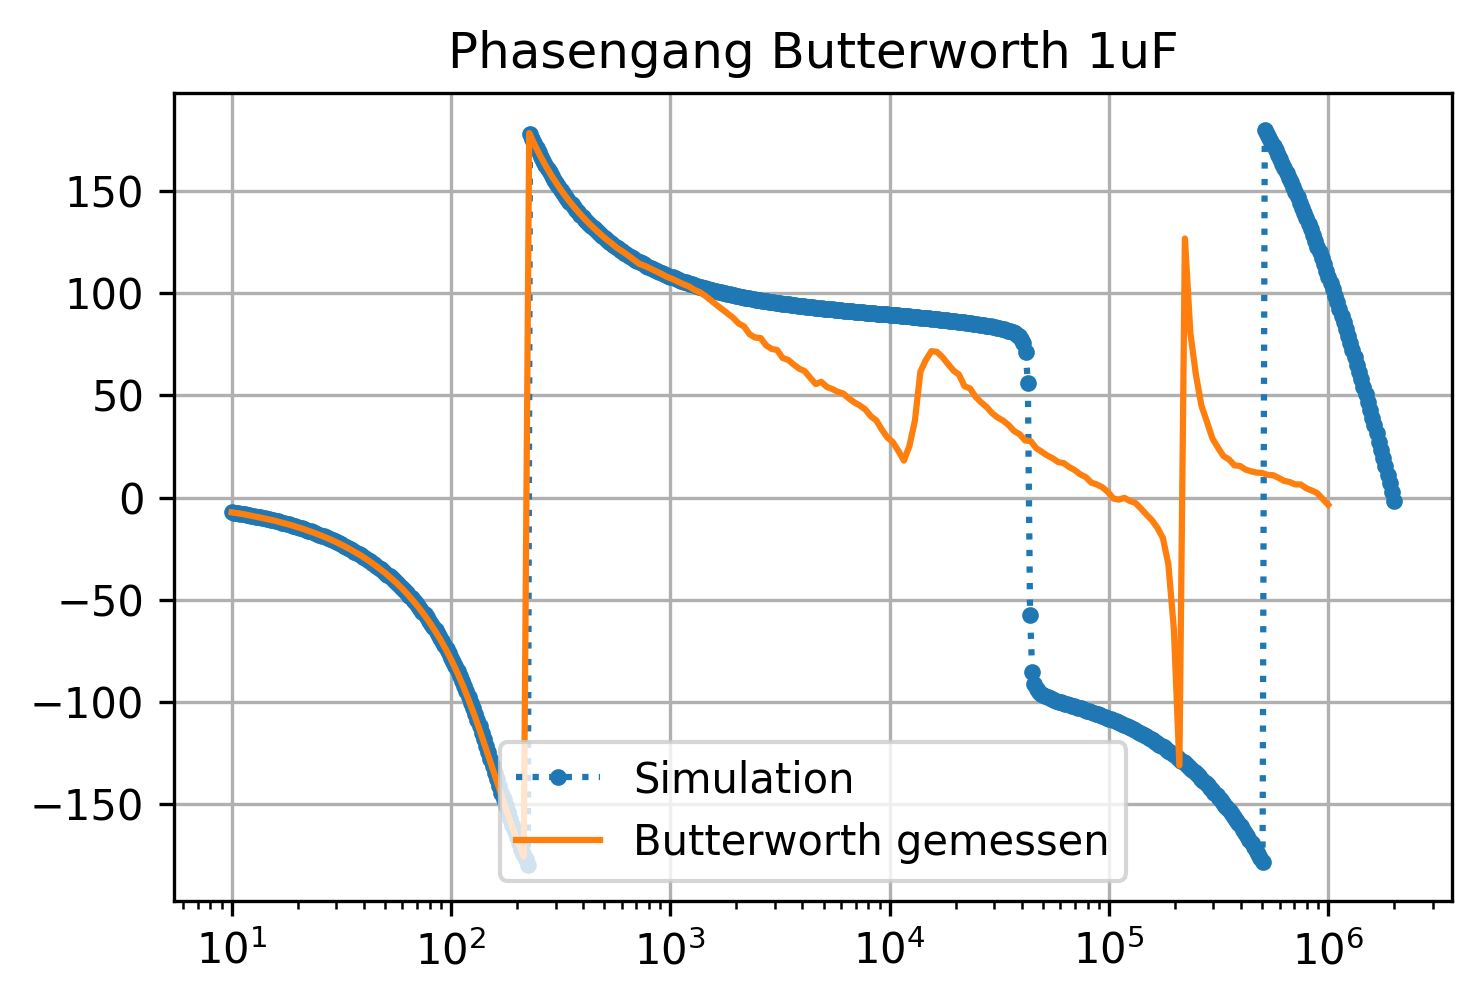
\includegraphics[keepaspectratio]{index_files/figure-pdf/cell-16-output-1.png}}

\subsection{Butterworthfilter 0.1uF}\label{butterworthfilter-0.1uf}

\begin{Shaded}
\begin{Highlighting}[]
\NormalTok{plt.figure(}\StringTok{"Amplitudengang Butterworth TP 0.1uF"}\NormalTok{)}
\NormalTok{plt.title(}\StringTok{"Amplitudengang Butterworth 0.1uF"}\NormalTok{)}
\NormalTok{plt.plot(f4,}\DecValTok{20}\OperatorTok{*}\NormalTok{np.log10(}\BuiltInTok{abs}\NormalTok{(Vout01u)),}\StringTok{".:"}\NormalTok{,label}\OperatorTok{=}\StringTok{"Simulation"}\NormalTok{)}
\NormalTok{plt.plot(fButter01uf,gain01uf,label}\OperatorTok{=}\StringTok{\textquotesingle{}Tiefpassfilter gemessen\textquotesingle{}}\NormalTok{)}
\NormalTok{plt.xscale(}\StringTok{\textquotesingle{}log\textquotesingle{}}\NormalTok{)}
\NormalTok{plt.grid()}
\NormalTok{plt.legend()}
\NormalTok{plt.show()}
\end{Highlighting}
\end{Shaded}

\pandocbounded{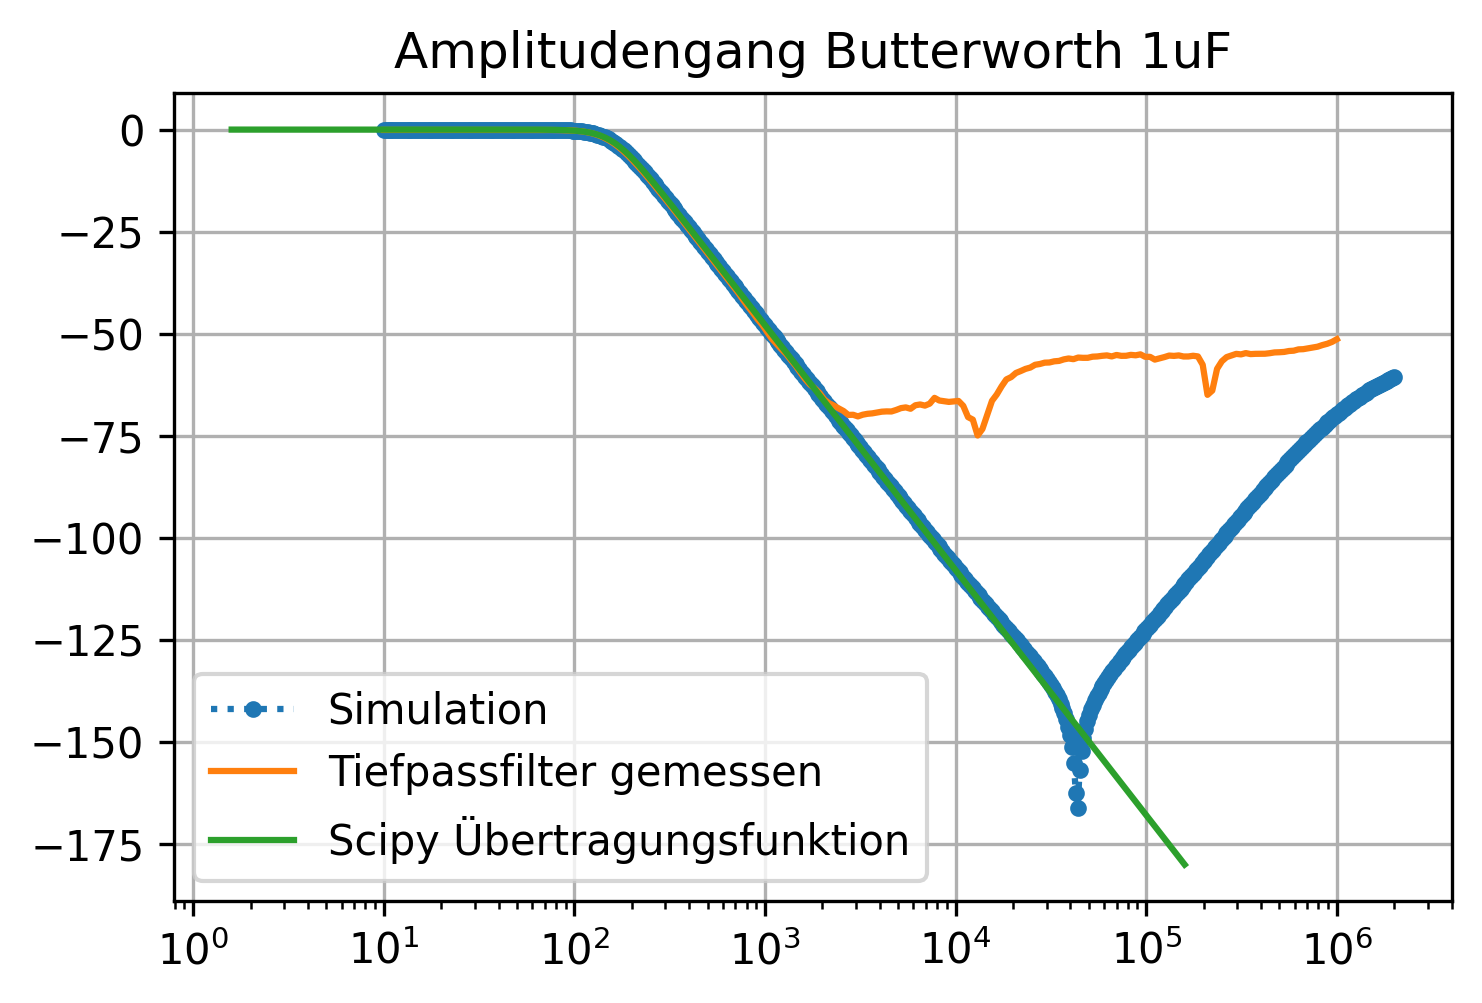
\includegraphics[keepaspectratio]{index_files/figure-pdf/cell-17-output-1.png}}

\begin{Shaded}
\begin{Highlighting}[]
\NormalTok{plt.figure(}\StringTok{"Phasengang Butterworth TP 0.1uF"}\NormalTok{)}
\NormalTok{plt.title(}\StringTok{"Phasengang Butterworth 0.1uF"}\NormalTok{)}
\NormalTok{plt.plot(f4,np.degrees(np.angle(Vout01u)),}\StringTok{".:"}\NormalTok{,label}\OperatorTok{=}\StringTok{"Simulation"}\NormalTok{)}
\NormalTok{plt.plot(fButter01uf,phase01uf,label}\OperatorTok{=}\StringTok{\textquotesingle{}Butterworth gemessen\textquotesingle{}}\NormalTok{)}
\NormalTok{plt.xscale(}\StringTok{\textquotesingle{}log\textquotesingle{}}\NormalTok{)}
\NormalTok{plt.grid()}
\NormalTok{plt.legend()}
\NormalTok{plt.show()}
\end{Highlighting}
\end{Shaded}

\pandocbounded{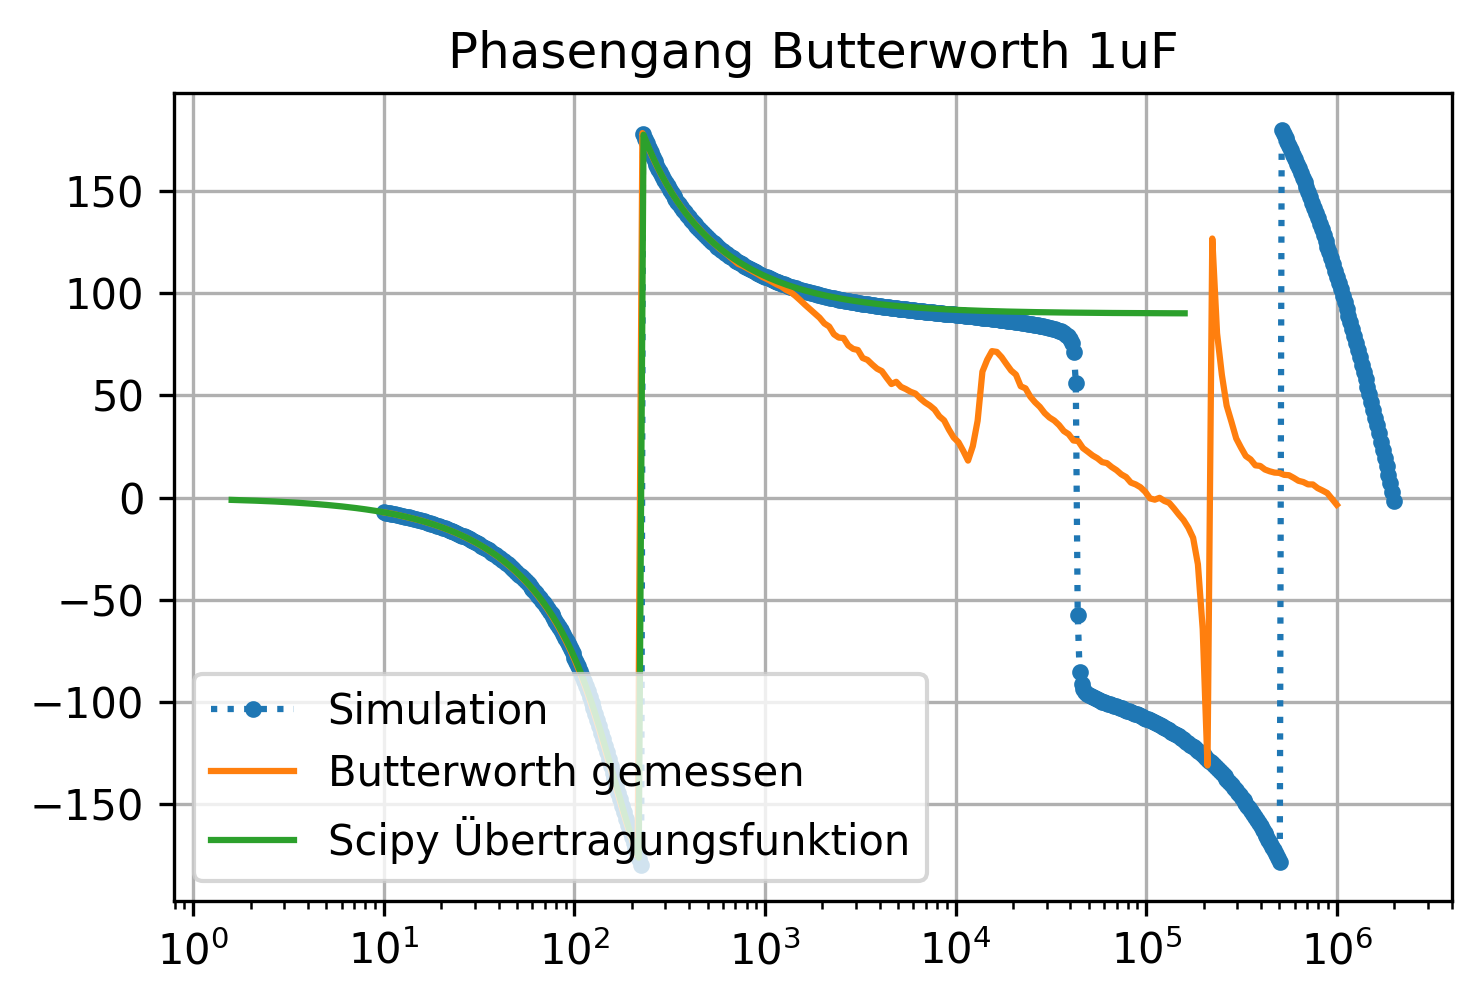
\includegraphics[keepaspectratio]{index_files/figure-pdf/cell-18-output-1.png}}

\subsection{Butterworthfilter 0.01uF}\label{butterworthfilter-0.01uf}

\begin{Shaded}
\begin{Highlighting}[]
\NormalTok{plt.figure(}\StringTok{"Amplitudengang Butterworth TP 0.01uF"}\NormalTok{)}
\NormalTok{plt.title(}\StringTok{"Amplitudengang Butterworth 0.01uF"}\NormalTok{)}
\NormalTok{plt.plot(f5,}\DecValTok{20}\OperatorTok{*}\NormalTok{np.log10(}\BuiltInTok{abs}\NormalTok{(Vout001u)),}\StringTok{".:"}\NormalTok{,label}\OperatorTok{=}\StringTok{"Simulation"}\NormalTok{)}
\NormalTok{plt.plot(fButter001uf,gain001uf,label}\OperatorTok{=}\StringTok{\textquotesingle{}Tiefpassfilter gemessen\textquotesingle{}}\NormalTok{)}
\NormalTok{plt.xscale(}\StringTok{\textquotesingle{}log\textquotesingle{}}\NormalTok{)}
\NormalTok{plt.grid()}
\NormalTok{plt.legend()}
\NormalTok{plt.show()}
\end{Highlighting}
\end{Shaded}

\pandocbounded{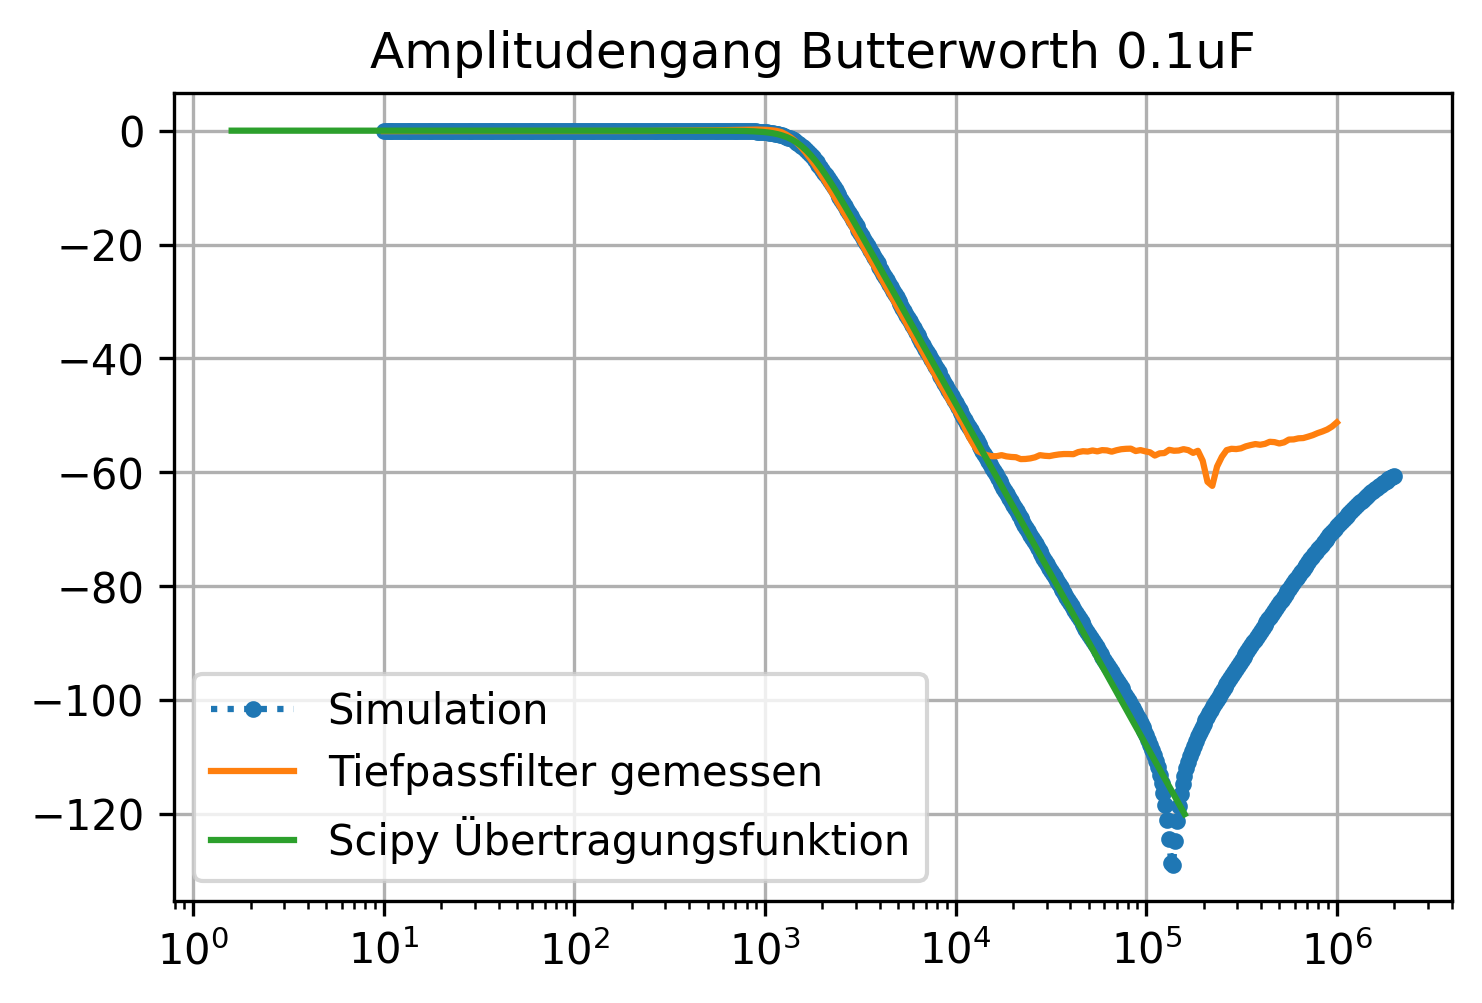
\includegraphics[keepaspectratio]{index_files/figure-pdf/cell-19-output-1.png}}

\begin{Shaded}
\begin{Highlighting}[]
\NormalTok{plt.figure(}\StringTok{"Phasengang Butterworth TP 0.01uF"}\NormalTok{)}
\NormalTok{plt.title(}\StringTok{"Phasengang Butterworth 0.01uF"}\NormalTok{)}
\NormalTok{plt.plot(f5,np.degrees(np.angle(Vout001u)),}\StringTok{".:"}\NormalTok{,label}\OperatorTok{=}\StringTok{"Simulation"}\NormalTok{)}
\NormalTok{plt.plot(fButter001uf,phase001uf,label}\OperatorTok{=}\StringTok{\textquotesingle{}Butterworth gemessen\textquotesingle{}}\NormalTok{)}
\NormalTok{plt.xscale(}\StringTok{\textquotesingle{}log\textquotesingle{}}\NormalTok{)}
\NormalTok{plt.grid()}
\NormalTok{plt.legend()}
\NormalTok{plt.show()}
\end{Highlighting}
\end{Shaded}

\pandocbounded{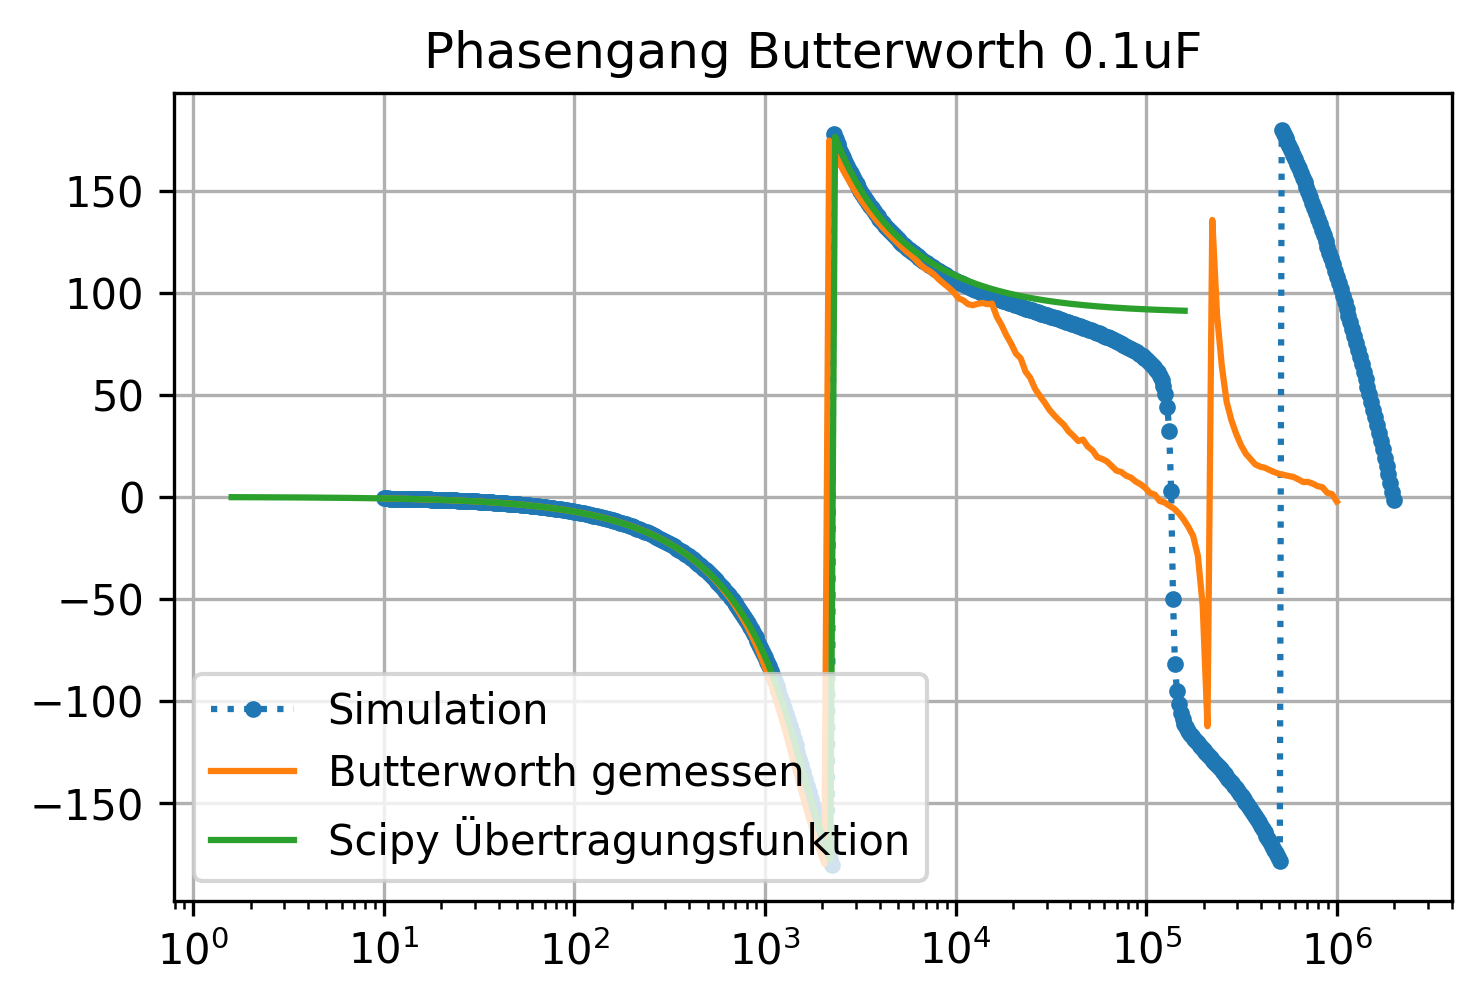
\includegraphics[keepaspectratio]{index_files/figure-pdf/cell-20-output-1.png}}

(Baker 2010)

\chapter{Entwurf der PCB Schaltung}\label{entwurf-der-pcb-schaltung}

\chapter*{Literaturverzeichnis}\label{literaturverzeichnis}
\addcontentsline{toc}{chapter}{Literaturverzeichnis}

\phantomsection\label{refs}
\begin{CSLReferences}{1}{0}
\bibitem[\citeproctext]{ref-baker2010}
Baker, R. Jacob. 2010. \emph{{CMOS}: Circuit Design, Layout, and
Simulation}. 3. Aufl. Wiley-IEEE Press.
\url{https://doi.org/10.1002/9780470891179}.

\end{CSLReferences}




\end{document}
